% This is a Basic Assignment Paper but with like Code and stuff allowed in it, there is also url, hyperlinks from contents included. 

\documentclass[openany]{report}

% Preamble

\usepackage[margin=1in]{geometry}
\usepackage{amsfonts, amsmath, amssymb}
\usepackage{fancyhdr, float, graphicx}
\usepackage[utf8]{inputenc} % Required for inputting international characters
\usepackage[T1]{fontenc} % Output font encoding for international characters
\usepackage{fouriernc} % Use the New Century Schoolbook font
\usepackage[nottoc, notlot, notlof]{tocbibind}
\usepackage{listings}
\usepackage{xcolor}
\usepackage{blindtext}
\usepackage{hyperref}
\usepackage{minted}

\hypersetup{
    colorlinks=true,
    linkcolor=black,
    filecolor=magenta,      
    urlcolor=blue,
    pdfpagemode=FullScreen,
    }

\definecolor{codegreen}{rgb}{0,0.6,0}
\definecolor{codegray}{rgb}{0.5,0.5,0.5}
\definecolor{codepurple}{rgb}{0.58,0,0.82}
\definecolor{backcolour}{rgb}{0.95,0.95,0.92}

\lstdefinestyle{mystyle}{
    backgroundcolor=\color{backcolour},   
    commentstyle=\color{codegreen},
    keywordstyle=\color{magenta},
    numberstyle=\tiny\color{codegray},
    stringstyle=\color{codepurple},
    basicstyle=\ttfamily\footnotesize,
    breakatwhitespace=false,         
    breaklines=true,                 
    captionpos=b,                    
    keepspaces=true,                 
    numbers=left,                    
    numbersep=5pt,                  
    showspaces=false,                
    showstringspaces=false,
    showtabs=false,                  
    tabsize=2
}

\lstset{style=mystyle}

% Header and Footer
\pagestyle{fancy}
\fancyhead{}
\fancyfoot{}
\fancyhead[L]{\textit{\Large{Blackbook - 4th Year B. Tech - Attendance Assistant}}}
\fancyhead[R]{\textit{Capstone}}
\fancyfoot[C]{\thepage}
\renewcommand{\footrulewidth}{1pt}

% Other Doc Editing
% \parindent 0ex
%\renewcommand{\baselinestretch}{1.5}

\begin{document}

% \begin{titlepage}
%     \centering

%     %---------------------------NAMES-------------------------------

%     \huge\textsc{
%         Dr. Vishwanath Karad MIT World Peace University, Pune
%     }\\

%     \vspace{0.75\baselineskip} % space after Uni Name

%     \LARGE{
%         Department of Computer Engineering \& Technology \\
%         School of Computer Science \& Engineering\\
%         Seminar\\
%         Year B. Tech, Semester 5\\
%     }

%     \vfill % space after Sub Name

%     %--------------------------TITLE-------------------------------

%     \rule{\textwidth}{1.6pt}\vspace*{-\baselineskip}\vspace*{2pt}
%     \rule{\textwidth}{0.6pt}
%     \vspace{0.75\baselineskip} % Whitespace above the title



%     \huge{\textsc{
%             Comparison between Face Recognition Algorithms and Techniques
%         }} \\



%     \vspace{0.5\baselineskip} % Whitespace below the title
%     \rule{\textwidth}{0.6pt}\vspace*{-\baselineskip}\vspace*{2.8pt}
%     \rule{\textwidth}{1.6pt}

%     \vspace{1\baselineskip} % Whitespace after the title block

%     %--------------------------SUBTITLE --------------------------	

%     \LARGE\textsc{
%         Seminar Report
%     } % Subtitle or further description

%     %--------------------------AUTHOR-------------------------------

%     \vspace{0.5\baselineskip} % Whitespace below the editor list
%     Under the Guidance of\\
%     \Large{
%         \textbf{Dr. Sharmishta Desai}
%     }
%     \vfill

%     Prepared By
%     \vspace{0.5\baselineskip} % Whitespace before the editors

%     \Large{
%         Krishnaraj Thadesar, PA10, 1032210888\\
%     }
%     \vspace{0.5\baselineskip} % Whitespace before the editors
%     % \vspace{0.5\baselineskip} % Whitespace below the editor list
%     \today

% \end{titlepage}
 
\chapter*{Acknowledgment}
\thispagestyle{empty}

I would like to express my deepest appreciation to all those who provided me the possibility to complete this report. A special gratitude I give to our mentor, \textbf{Dr. Sharmishta Desai}, whose contribution in stimulating suggestions and encouragement, helped me to coordinate my project especially in writing this report.\\

Furthermore, I would also like to acknowledge with much appreciation the crucial role of the staff of MIT WPU, who gave the permission to use all required equipment and the necessary materials to complete the task. A special thanks goes to my team mates,who helped me enormously to assemble the parts and gave suggestion about the task of using the techniques of measurements.\\

I have to appreciate the guidance given by other supervisor as well as the panels especially in our project presentation that has improved our presentation skills thanks to their comment and advices.\\

I would also like to thank my parents for their wise counsel and sympathetic ear. You are always there for me. Finally, I wish to thank my friends for their support and encouragement throughout my study.

\vspace{5cm}

\begin{flushright}
    \section*{Name of Students}
    \begin{tabular}{r}
   Krishnaraj Thadesar, 1032210888 \\
   Parth Zarekar, 1032210846 \\
   Sourab Karad, 1032211150 \\
   Saubhagya Singh, 1032211144 \\
    \end{tabular}
    \end{flushright}
    
\thispagestyle{empty}
\clearpage

\chapter*{Abstract}
The Attendance-Assistant project introduces an innovative, cross-platform mobile application designed to automate attendance tracking in educational institutions using advanced facial recognition technology. The system leverages Flutter for the frontend, ensuring a seamless and intuitive user experience, while the backend is powered by FastAPI and MongoDB, providing robust, secure, and scalable data management. This comprehensive solution streamlines the entire attendance workflow, encompassing user authentication, face-encoding management, real-time attendance marking, and detailed reporting.\\ 


This report documents the systematic approach undertaken to evaluate and compare various face recognition algorithms, focusing on their precision metrics, computational efficiency, and real-world applicability. After rigorous testing, the ResNet-based implementation in Python, utilizing the \textit{face\_recognition} library, was selected for its superior accuracy and reliability. The report further elaborates on the system architecture, database schema, and core functionalities, highlighting how the Attendance-Assistant enhances operational efficiency, accuracy, and user convenience compared to traditional attendance methods.\\


The project also explores the integration of IoT devices, such as Raspberry Pi, to enable real-time facial recognition in classrooms and other institutional settings. By combining cutting-edge technologies with a user-centric design, the Attendance-Assistant aims to revolutionize attendance management, offering a scalable and efficient solution for modern educational institutions.

\section*{Keywords}
Facial Recognition, Attendance Automation, Flutter, FastAPI, MongoDB, ResNet, Educational Institutions, IoT, Raspberry Pi, Backend Development, Frontend Development, Data Integrity, Firebase, Precision Metrics, Attendance Management System

\listoffigures
\clearpage
\listoftables
\clearpage

\tableofcontents
\thispagestyle{empty}
\clearpage
 
\chapter{Introduction}

Face recognition is a biometric technology that utilizes distinctive features of the face to identify individuals. Widely employed in security systems, it serves various applications such as access control, attendance tracking, and surveillance. While face recognition has existed for decades, recent advancements in machine learning and computer vision have significantly enhanced its accuracy and reliability. Numerous algorithms and techniques are available, each with unique strengths and weaknesses. In this seminar, we aim to compare popular face recognition algorithms and assess their performance using a standardized dataset.

\subsection{Problem Statement}
We need to compare the various face recognition algorithms and techniques to determine which one is the most accurate and efficient. We also need to discuss the implementation of these algorithms in real-world applications.

\subsection{Need of the Project}

\begin{itemize}
    \item The motivation for this topic came from impending research for a Project titled "Machine Learning Powered Automated Facial Attendance Tracking System".
    \item The project aims to develop a system that can automatically track attendance using facial recognition technology.
    \item To achieve this goal, it is essential to understand the different face recognition algorithms and techniques available and evaluate their performance to identify the most suitable approach for the project.
    \item By comparing the performance of different face recognition algorithms and techniques, we can gain insights into their strengths and weaknesses and make informed decisions about which approach to use for the project.
    \item This seminar will provide a comprehensive overview of the most popular face recognition algorithms and techniques and evaluate their performance on a common dataset to help guide the development of the attendance tracking system.
\end{itemize}

This project will help in understanding the various face recognition algorithms and techniques and how they can be implemented in real-world applications. It will also help in understanding the challenges faced in face recognition and how these challenges can be overcome.

To use the correct method and library in finding attendance, so as to reduce time and cost, while also maintaining high levels of accuracy, it was necessary to compare the various face recognition algorithms and techniques.

\chapter{Literature Survey}

\section{Paper 1}
Title:  \textit{"A Comparative Study of Facial Recognition Techniques: With focus on low computational power."}
Author:  \textit{Schenkel, T., Ringhage, O. and Branding, N.}
\cite{7}
\subsection{Positives and Learnings from this Paper}

\begin{enumerate}
    \item {The publication compares five performance metrics, including recall and F-score, providing a comprehensive evaluation of facial recognition techniques.}
    \item {It addresses the importance of balancing low computational time and prediction ability for security systems, offering practical guidelines for implementation.}
    \item {The research questions are clearly defined, focusing on significant differences in performance, training time, and prediction time among different facial recognition techniques and classifiers.}
\end{enumerate}
\subsection{Identified Research Gaps}

\begin{enumerate}
    \item The document lacks detailed information on the specific facial recognition techniques and classifiers used in the experiments.
    \item It does not provide a detailed breakdown of the dataset used for training and testing the facial recognition models.
    \item While the document mentions the comparison of results, it does not delve into the specific findings or implications of these comparisons.
\end{enumerate}

\section{Paper 2}
Title:  \textit{"A Comparative Study on Facial Recognition Algorithms"}
Author:  \textit{Sanmoy Paul and Sameer Acharya}
\cite{8}

\subsection{Positives and Learnings from this Paper}
\begin{enumerate}
    \item Comparative Analysis: The study provides a comparative analysis of different facial recognition algorithms, allowing developers to make informed choices based on recognition accuracies.

    \item Algorithm Selection: By studying the advantages and disadvantages of various algorithms, developers can select the best facial recognition algorithm for their specific implementation needs.

    \item Future Improvements: The research suggests future efforts to test on a larger set of images to enhance the accuracy of CNN and explore combining multiple machine learning classification algorithms for increased recognition accuracy and handling large datasets.
\end{enumerate}
\subsection{Identified Research Gaps}

\begin{enumerate}
    \item The document lacks detailed discussion on the specific methodologies used for training and testing the algorithms, which could provide more clarity on the experimental setup.
    \item There is no mention of the computational resources or hardware specifications used for running the experiments, which could impact the reproducibility and scalability of the results.
    \item The publication does not delve into the potential biases or limitations in the dataset used for training and testing the facial recognition models, which could affect the generalizability of the findings.
\end{enumerate}

\section{Paper 3}
Title:  \textit{"A comparison of facial recognition algorithms."}
Author:  \textit{Delbiaggio, Nicolas. }
\cite{9}
\subsection{Positives and Learnings from this Paper}
\begin{enumerate}
    \item Thesis covers a comprehensive comparison of facial recognition algorithms like Eigenfaces, Fisherfaces, LBPH, and OpenFace.

    \item The study includes a detailed explanation of each algorithm, their strengths, weaknesses, and performance in a test case scenario.

    \item The findings highlight OpenFace as the most accurate algorithm for facial recognition, providing valuable insights for further research in the field.
\end{enumerate}
\subsection{Identified Research Gaps}
\begin{enumerate}
    \item Lack of Exploration of Real-World Applications: The paper focuses on comparing facial recognition algorithms in a controlled setting. However, it does not delve into the practical applications of these algorithms in real-world scenarios.

    \item Limited Discussion on Algorithm Limitations: While the strengths of the algorithms are discussed, there is a lack of emphasis on the limitations of each algorithm.

    \item Absence of Future Research Directions: The paper concludes with the identification of the most accurate algorithm but fails to suggest potential future research directions in the field of facial recognition.
\end{enumerate}

\section{Paper 4}
Title:  \textit{"Evaluating impact of race in facial recognition across machine learning and deep learning algorithms."}
Author:  \textit{Coe, James, and Mustafa Atay.}
\cite{10}
\subsection{Positives and Learnings from this Paper}
\begin{enumerate}
    \item The paper provides a detailed comparison of various facial recognition algorithms, including Eigenfaces, Fisherfaces, Local Binary Pattern Histogram, deep convolutional neural network algorithm, and OpenFace.
    \item It highlights the efficiency and accuracy of these algorithms in real-life settings, with OpenFace being identified as the algorithm with the highest accuracy in identifying faces.
    \item The study's findings offer valuable insights for practitioners in selecting the most suitable algorithm for facial recognition applications and suggest ways for academicians to enhance the current algorithms' accuracy further.
\end{enumerate}
\subsection{Identified Research Gaps}
\begin{enumerate}
    \item The paper focuses on a few specific facial recognition algorithms like Eigenfaces, Fisherfaces, and Local Binary Pattern Histograms. It lacks exploration of a wider range of algorithms available in the field, potentially missing out on newer, more accurate models.

    \item While the study evaluates the algorithms' accuracy, it does not delve into their performance in real-life settings or practical applications. This gap could impact the algorithms' effectiveness when deployed in scenarios beyond controlled test environments.

    \item The paper mentions the use of a custom dataset for testing the algorithms but does not elaborate on the dataset's diversity or size.
\end{enumerate}

\section{Paper 5}

Title:  \textit{"A Comparative Study of Facial Recognition Techniques: With focus on low computational power."}
Author:  \textit{Schenkel, T., Ringhage, O. and Branding, N.} \cite{11}
\subsection{Positives and Learnings from this Paper}

\begin{enumerate}
    \item Efficiency Evaluation: The paper provides a detailed comparison of popular open source facial recognition algorithms, highlighting the efficiency and accuracy of each in real-life settings.

    \item Practical Implications: The findings of the study offer valuable insights for practitioners in selecting the most suitable algorithm for facial recognition applications, enhancing decision-making processes.

    \item Academic Contribution: The research contributes to the academic field by emphasizing the importance of improving the accuracy of existing algorithms, paving the way for further advancements in facial recognition technology.
\end{enumerate}

\subsection{Identified Research Gaps}
\begin{enumerate}
    \item The paper focuses on comparing a few facial recognition algorithms like Eigenfaces, Fisherfaces, and Local Binary Pattern Histogram. However, it lacks a comparison with a wider range of algorithms to provide a more comprehensive analysis.

    \item While the paper evaluates the algorithms' performance in a controlled environment using test datasets, it doesn't discuss the practical implementation challenges or results in real-life scenarios, which could be a crucial research gap.

    \item The paper does not delve into the scalability and efficiency aspects of the facial recognition algorithms studied. Understanding how these algorithms perform with larger datasets or in real-time applications could be a significant research gap to address.
\end{enumerate}

\chapter{Problem Statement}

Manual attendance tracking at MITWPU Campus is a time-consuming process prone to inefficiencies and potential malpractices. The current system lacks automation, leading to increased per-class time spent on attendance management.
	\vspace*{0.5cm}
	To address these challenges, there is a need for the development of an Automated Attendance Tracking System. The solution should leverage computer vision for accurate data capture, utilize cloud infrastructure for efficient storage and processing, and incorporate advanced data science techniques for analytics.

	\vspace*{0.5cm}
	The system should be user-friendly, providing both teachers and students with a seamless experience while ensuring security and tamper resistance to mitigate the risk of malpractices in attendance tracking. The goal is to enhance overall efficiency and significantly reduce the manual effort involved in attendance monitoring.

\section{Project Scope}

The scope of the project includes the following key components:

\begin{enumerate}
    \item Development of a mobile application using Flutter for user interaction and attendance management.
    \item Implementation of a backend system using FastAPI for handling API requests and data processing.
    \item Integration of a cloud database (MongoDB) for secure and scalable data storage.
    \item Utilization of computer vision techniques for real-time face recognition and attendance marking.
\end{enumerate}

\section{Project Assumptions}

\begin{enumerate}
    \item The system will be used in a controlled environment, such as a classroom or lecture hall, where the lighting and camera angles are optimal for face recognition.
    \item Users will have access to the necessary hardware and software components required for the system to function effectively.
    \item The system will be used primarily for attendance tracking purposes and not for any other applications.
    \item Users will have basic knowledge of using mobile applications and web interfaces.
    \item The system will comply with relevant data privacy regulations and guidelines.
    
\end{enumerate}
\section{Project Limitations}

\begin{enumerate}
    \item Privacy Concerns: Face recognition technology raises privacy concerns due to its potential for misuse and abuse.
    \item Security Risks: Face recognition systems can be vulnerable to attacks, such as spoofing and impersonation, which can compromise security.
    \item Bias and Discrimination: Face recognition systems can be biased and discriminatory, leading to inaccurate and unfair results.
    \item Legal and Ethical Issues: Face recognition technology raises legal and ethical issues related to data privacy, consent, and surveillance.
    \item Technical Limitations: Face recognition technology has technical limitations, such as sensitivity to variations in lighting, pose, and occlusions, which can affect accuracy and reliability.\item
\end{enumerate}
\section{Project Objectives}

\begin{enumerate}
    \item Develop an automated attendance tracking system using computer vision for any organization
    \item Utilize cloud infrastructure for efficient storage and processing of attendance data.
    \item Create a user-friendly application for both teachers and students to simplify attendance management.
    \item Implement advanced data science techniques for processing large attendance datasets and performing analytics.
    \item Significantly reduce per-class time spent on attendance tracking through automated processes, enhancing overall efficiency.
    \item Mitigate the risk of malpractices in attendance tracking by implementing secure and tamper-resistant mechanisms.
\end{enumerate}
\chapter{Project Requirements}

\section{Requirements}
\subsection{Hardware Requirements}
\begin{table}[h!]
    \centering
    \begin{tabular}{|l|p{8cm}|r|}
    \hline
    \textbf{Name} & \textbf{Purpose} & \textbf{Cost (INR)} \\
    \hline
    Raspberry Pi Hi Quality Camera & Official camera from Raspberry Pi, more expensive for high resolution. & 8000 \\
    \hline
    Raspberry Pi Camera Module 3 & Official camera from Raspberry Pi, cheaper and highest resolution for cheapest cost. & 3000 \\
    \hline
    Raspberry Pi 4 Model B with 2 GB RAM & To send image from camera to server. & 5000 \\
    \hline
    \end{tabular}
    \caption{List of Hardware Requirements}
    \label{tab:hardware_requirements}
\end{table}
\subsection{Software Requirements}

\begin{enumerate}
    \item Amazon S3
\item Amazon EC2
\item Amazon DynamoDB
\item Raspian OS
\item Python Libraries

\end{enumerate}

\begin{lstlisting}
annotated-types==0.6.0
anyio==4.2.0
argon2-cffi==23.1.0
argon2-cffi-bindings==21.2.0
arrow==1.3.0
asttokens==2.4.1
async-lru==2.0.4
attrs==23.2.0
Babel==2.14.0
beautifulsoup4==4.12.3
bleach==6.1.0
CacheControl==0.14.0
cachetools==5.3.2
certifi==2024.2.2
cffi==1.16.0
charset-normalizer==3.3.2
click==8.1.7
colorama==0.4.6
comm==0.2.1
contourpy==1.2.0
cryptography==42.0.5
cycler==0.12.1
debugpy==1.8.1
decorator==5.1.1
defusedxml==0.7.1
dlib==19.24.2
dnspython==2.6.1
exceptiongroup==1.2.0
executing==2.0.1
face-recognition==1.3.0
face_recognition_models==0.3.0
fastapi==0.109.2
fastjsonschema==2.19.1
firebase-admin==6.4.0
fonttools==4.49.0
fqdn==1.5.1
gcloud==0.18.3
google-api-core==2.17.1
google-api-python-client==2.119.0
google-auth==2.28.1
google-auth-httplib2==0.2.0
google-cloud-core==2.4.1
google-cloud-firestore==2.15.0
google-cloud-storage==2.14.0
google-crc32c==1.5.0
google-resumable-media==2.7.0
googleapis-common-protos==1.62.0
grpcio==1.62.0
grpcio-status==1.62.0
h11==0.14.0
httpcore==1.0.4
httplib2==0.22.0
httpx==0.27.0
idna==3.6
ipykernel==6.29.2
ipython==8.21.0
ipywidgets==8.1.2
isoduration==20.11.0
jedi==0.19.1
Jinja2==3.1.3
json5==0.9.17
jsonpointer==2.4
jsonschema==4.21.1
jsonschema-specifications==2023.12.1
jupyter==1.0.0
jupyter-console==6.6.3
jupyter-events==0.9.0
jupyter-lsp==2.2.2
jupyter_client==8.6.0
jupyter_core==5.7.1
jupyter_server==2.12.5
jupyter_server_terminals==0.5.2
jupyterlab==4.1.2
jupyterlab_pygments==0.3.0
jupyterlab_server==2.25.3
jupyterlab_widgets==3.0.10
jwcrypto==1.5.4
kiwisolver==1.4.5
MarkupSafe==2.1.5
matplotlib==3.8.3
matplotlib-inline==0.1.6
mistune==3.0.2
msgpack==1.0.7
nbclient==0.9.0
nbconvert==7.16.1
nbformat==5.9.2
nest-asyncio==1.6.0
notebook==7.1.0
notebook_shim==0.2.4
numpy==1.26.4
oauth2client==4.1.3
opencv-python==4.9.0.80
overrides==7.7.0
packaging==23.2
pandocfilters==1.5.1
parso==0.8.3
pillow==10.2.0
pipdeptree==2.16.0
platformdirs==4.2.0
prometheus_client==0.20.0
prompt-toolkit==3.0.43
proto-plus==1.23.0
protobuf==4.25.3
psutil==5.9.8
pure-eval==0.2.2
pyasn1==0.5.1
pyasn1-modules==0.3.0
pycparser==2.21
pycryptodome==3.20.0
pydantic==2.5.3
pydantic_core==2.14.6
Pygments==2.17.2
PyJWT==2.8.0
pymongo==4.6.2
pyparsing==3.1.1
python-dateutil==2.8.2
python-dotenv==1.0.1
python-json-logger==2.0.7
python-jwt==4.1.0
python-multipart==0.0.9
pywin32==306
pywinpty==2.0.12
PyYAML==6.0.1
pyzmq==25.1.2
qtconsole==5.5.1
QtPy==2.4.1
referencing==0.33.0
requests==2.29.0
requests-toolbelt==0.10.1
rfc3339-validator==0.1.4
rfc3986-validator==0.1.1
rpds-py==0.18.0
rsa==4.9
Send2Trash==1.8.2
services==0.1.1
six==1.16.0
sniffio==1.3.0
soupsieve==2.5
stack-data==0.6.3
starlette==0.37.1
terminado==0.18.0
tinycss2==1.2.1
tomli==2.0.1
tornado==6.4
traitlets==5.14.1
types-python-dateutil==2.8.19.20240106
typing_extensions==4.9.0
uri-template==1.3.0
uritemplate==4.1.1
urllib3==1.26.18
uvicorn==0.27.0
wcwidth==0.2.13
webcolors==1.13
webencodings==0.5.1
websocket-client==1.7.0
widgetsnbextension==4.0.10

\end{lstlisting}

\section{Risk Management}
\begin{enumerate}
    \item \textbf{Technical Risks}: The project may face technical challenges related to the integration of various components, such as the mobile application, backend, and cloud services. To mitigate this risk, thorough testing and validation will be conducted at each stage of development.
    \item \textbf{Data Privacy Risks}: The use of face recognition technology raises concerns about data privacy and security. To address this, the system will comply with relevant data protection regulations and implement secure data storage and transmission practices.
    \item \textbf{User Acceptance Risks}: Users may be resistant to adopting the new system due to concerns about privacy or usability. To mitigate this risk, user training and support will be provided, along with clear communication about the benefits of the system.
    \item \textbf{Performance Risks}: The system may not perform as expected under high load or in real-world conditions. To address this, performance testing will be conducted to ensure the system can handle the expected number of users and data volume.
    \item \textbf{Regulatory Risks}: Changes in regulations related to data privacy and face recognition technology may impact the project. To mitigate this risk, the project team will stay informed about relevant regulations and adapt the system as needed to ensure compliance.
\end{enumerate}
\section{Functional Specifications}
\subsection{Interfaces}

\subsubsection{External Interfaces Required}
\begin{enumerate}
    \item \textbf{User Interface}: The mobile application will have a user-friendly interface for students and teachers to interact with the system. It will include features for face capture, attendance marking, and viewing attendance history.
    \item \textbf{Camera Interface}: The system will utilize the camera on the mobile device or an external camera (e.g., Raspberry Pi camera) for face capture. The camera will be integrated with the mobile application to capture images for face recognition.
    \item \textbf{Cloud Storage}: The system will use cloud storage (e.g., AWS S3) for storing images and other media files. The backend will handle the upload and retrieval of these files.
    \item \textbf{Database Interface}: The system will connect to a cloud database (e.g., MongoDB Atlas) for storing user data, face encodings, and attendance records. The backend will interact with the database to perform CRUD operations.
    \item \textbf{IoT Device Interface}: If IoT devices (e.g., Raspberry Pi) are used for real-time face recognition, they will communicate with the backend via HTTP requests to send captured images and receive attendance updates.
\end{enumerate}
\subsubsection{Internal Interfaces Required}
\begin{enumerate}
    \item \textbf{Frontend}: The mobile application will be developed using Flutter, which will communicate with the backend via RESTful APIs. The frontend will handle user authentication, face capture, and attendance display.
    \item \textbf{Backend}: The backend will be developed using FastAPI, which will handle API requests from the frontend. It will also manage face encoding and attendance logging. The backend will connect to the MongoDB database for data storage and retrieval.
    \item \textbf{Database}: The MongoDB database will store user data, face encodings, and attendance records. The backend will interact with the database to perform CRUD operations.
\end{enumerate}
\subsubsection{Communication Interfaces}
\begin{enumerate}
    \item \textbf{REST API}: The system will use RESTful APIs for communication between the frontend and backend components. The APIs will handle requests for user authentication, face encoding, and attendance logging.
    \item \textbf{Database Connection}: The backend will connect to the MongoDB database using a secure connection string. The database will store user data, face encodings, and attendance records.
    \item \textbf{Cloud Storage}: The system will use cloud storage (e.g., AWS S3) for storing images and other media files. The backend will handle the upload and retrieval of these files.
    \item \textbf{IoT Device Communication}: If IoT devices (e.g., Raspberry Pi) are used for real-time face recognition, they will communicate with the backend via HTTP requests to send captured images and receive attendance updates.
    \item \textbf{User Authentication}: The system will implement user authentication using JWT (JSON Web Tokens) for secure access to the APIs. Users will need to log in to access the attendance features.
\end{enumerate}
\subsubsection{Graphical User Interfaces}
\begin{figure}[H]
    \centering
    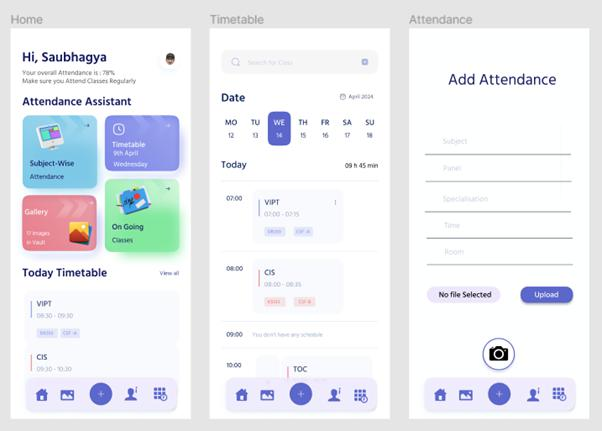
\includegraphics[width=.95\textwidth]{../imgs/app 2.jpg}
    \caption{App Design}
\end{figure}

\begin{figure}[H]
    \centering
    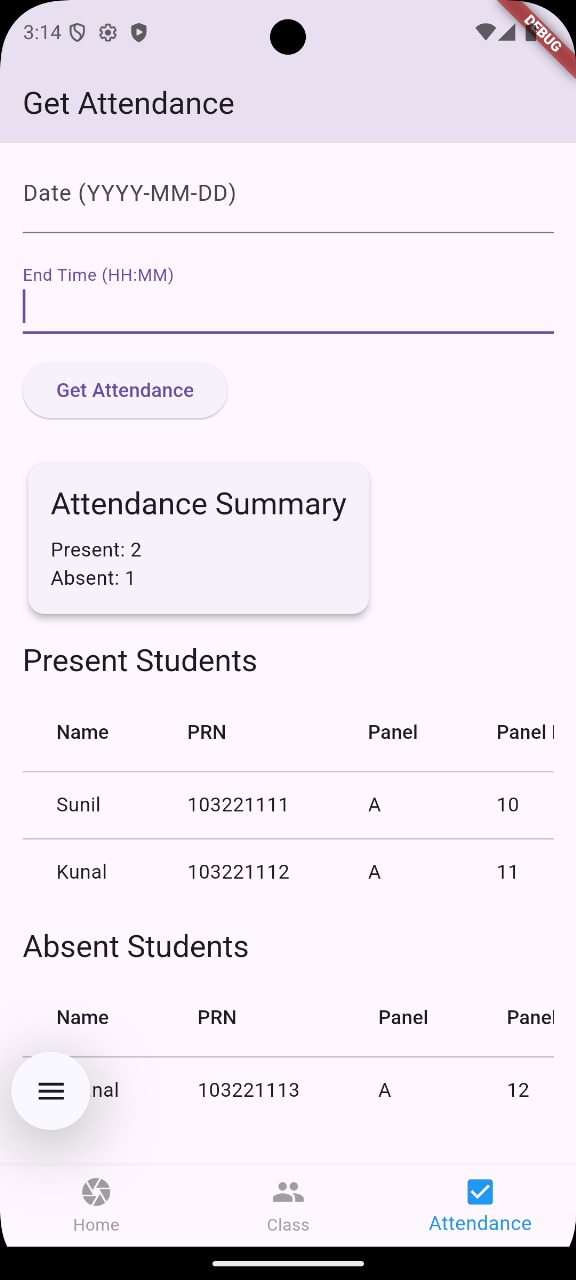
\includegraphics[width=.95\textwidth]{../imgs/app 3.jpg}
    \caption{App Design}
\end{figure}
\subsection{Interactions}
\subsubsection{Sustainability}
\begin{enumerate}
    \item The system will be designed to be scalable, allowing for easy addition of new features and functionalities in the future.
    \item The use of cloud services will ensure that the system can handle increased data storage and processing requirements as the user base grows.
    \item The system will be developed using modular architecture, making it easier to maintain and update individual components without affecting the entire system.
    \item The project will follow best practices in software development, including version control, code reviews, and documentation, to ensure long-term maintainability.
\end{enumerate}
\subsubsection{Quality Management}
\begin{enumerate}
    \item The system will undergo rigorous testing, including unit tests, integration tests, and user acceptance tests, to ensure high quality and reliability.
    \item The project will follow coding standards and best practices to maintain code quality and readability.
    \item The system will implement error handling and logging mechanisms to identify and resolve issues quickly.
    \item The project will include documentation for both developers and users, providing clear instructions on how to use and maintain the system.
\end{enumerate}
\subsubsection{Security}

\begin{enumerate}
    \item The system will implement secure user authentication using JWT (JSON Web Tokens) to protect user data and prevent unauthorized access.
    \item All sensitive data, including user credentials and face encodings, will be encrypted before being stored in the database.
    \item The system will use HTTPS for secure communication between the frontend and backend components, ensuring that data transmitted over the network is encrypted.
    \item The project will follow best practices for data privacy and compliance with relevant regulations, such as GDPR, to protect user information.
    \item The system will implement access controls to restrict access to sensitive data and functionalities based on user roles (e.g., admin, teacher, student).
    \item The project will include regular security audits and vulnerability assessments to identify and address potential security risks.
    \item The system will implement logging and monitoring mechanisms to track user activities and detect any suspicious behavior.
\end{enumerate}


\chapter{System Analysis Proposed Architecture}

\section{Block Diagram}
\begin{figure}[H]
    \centering
    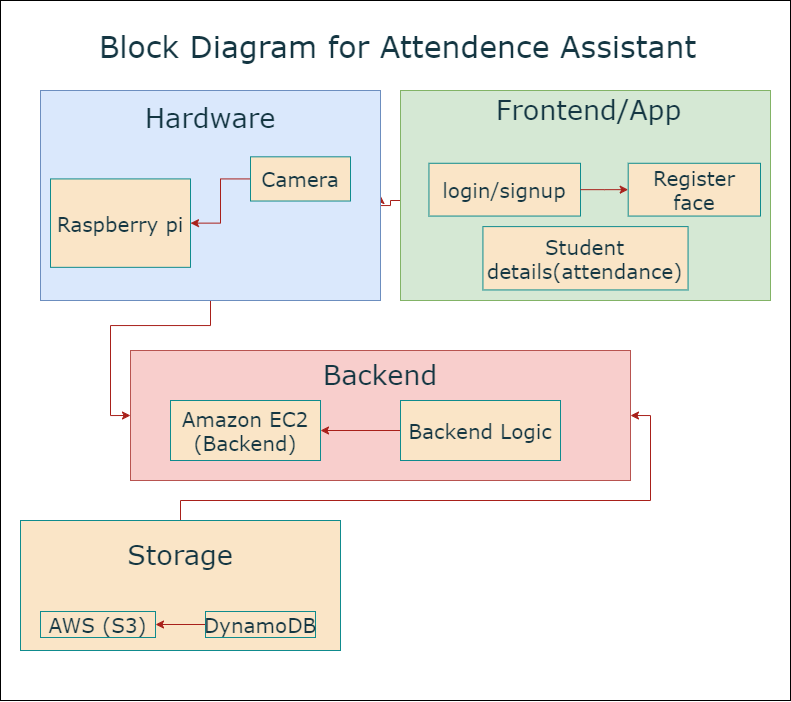
\includegraphics[width=.75\textwidth]{../imgs/block diagram.png}
    \caption{Block Diagram}
\end{figure}

\section{Activity Diagram}
\begin{figure}[H]
    \centering
    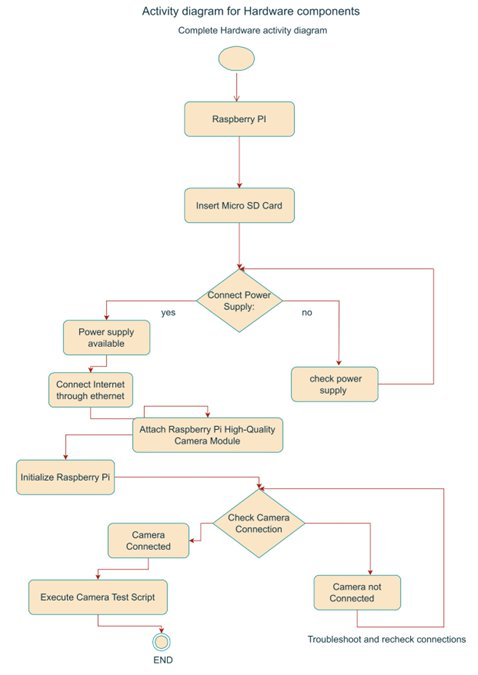
\includegraphics[width=.95\textwidth]{../imgs/activity 1.jpg}
    \caption{Activity Diagram}
\end{figure}

\begin{figure}[H]
    \centering
    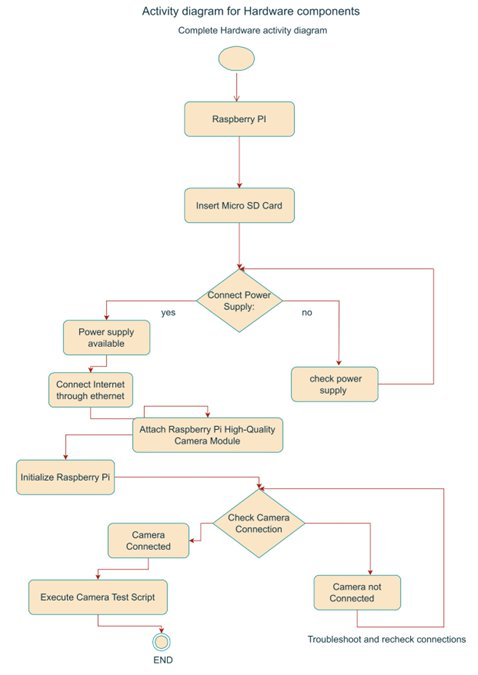
\includegraphics[width=.95\textwidth]{../imgs/activity 2.jpg}
    \caption{Activity Diagram Continued}
\end{figure}

\chapter{Project Plan - Timeline}
\begin{figure}[H]
    \centering
    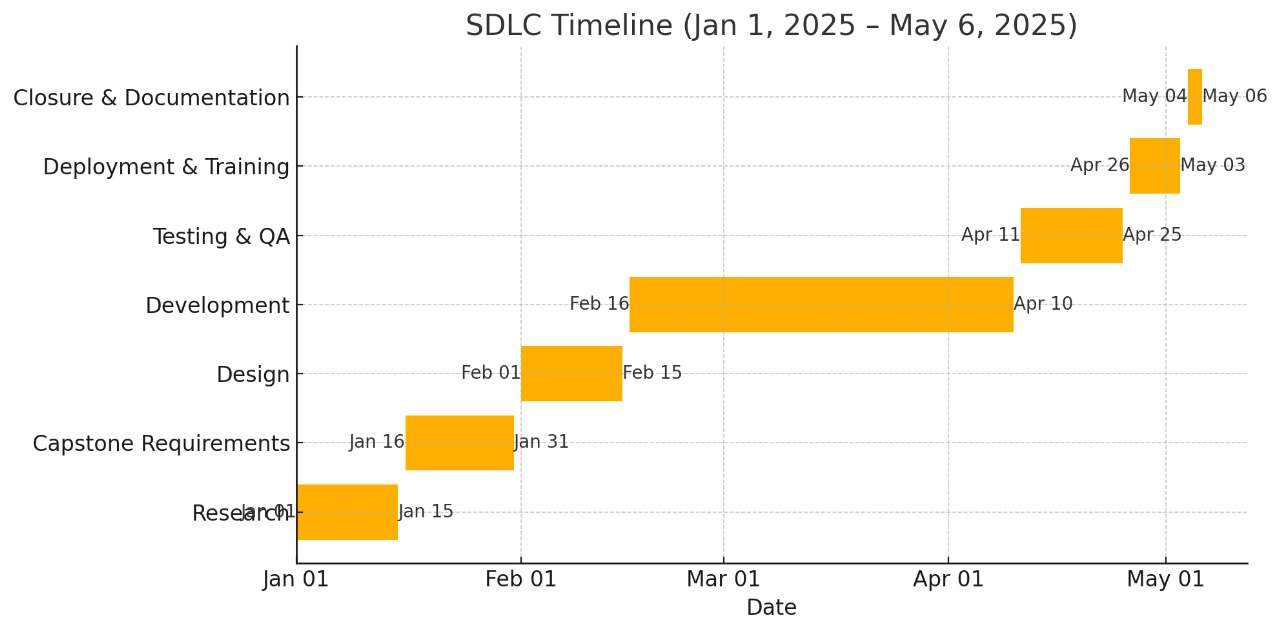
\includegraphics[width=.95\textwidth]{../imgs/timeline.jpg}
    \caption{Project Timeline}
\end{figure}


\section{Phase 1: Research}

\begin{enumerate}
    \item We started with a literature survey to understand the existing face recognition algorithms and their performance metrics.
    \item We compared the performance of different algorithms, including Eigenfaces, Fisherfaces, LBPH, and OpenFace, to identify the most suitable one for our project.
    \item We also explored the use of deep learning techniques, such as Convolutional Neural Networks (CNNs), for face recognition.
    \item 
\end{enumerate}

\section{Phase 2: Requirements Gathering}

\begin{enumerate}
    \item Conducted stakeholder interviews with professors and students to understand their pain points in attendance tracking.
    \item Defined use cases such as "Mark attendance for a class of 50 students in under 5 minutes" and "Generate attendance reports for a semester."
    \item Identified non-functional requirements like 95\% accuracy, real-time processing, and GDPR compliance for data privacy.
    \item Created a requirements traceability matrix to map user stories to functional and non-functional requirements.
\end{enumerate}

\section{Phase 3: System and Architecture Design}

\begin{enumerate}
    \item Designed a modular architecture with three main components: frontend (Flutter), backend (FastAPI), and database (MongoDB).
    \item Created a system block diagram showing data flow between the mobile app, API, and database.
    \item Defined REST API endpoints for user authentication, face encoding, and attendance logging.
    \item Developed a database schema with collections for users, face encodings, and attendance logs.
    \item Incorporated fault-tolerant mechanisms like retry logic for API calls and database backups.
\end{enumerate}

\section{Phase 4: Development}

\begin{enumerate}
    \item Implemented the backend using FastAPI, including endpoints for face encoding and attendance marking.
    \item Developed the frontend using Flutter, with features like face capture, attendance history, and user authentication.
    \item Integrated the face\_recognition library for face detection and recognition in the backend.
    \item Used Docker to containerize the application for consistent deployment across environments.
    \item Followed Git flow for version control, with feature branches and pull requests for code reviews.
\end{enumerate}

\section{Phase 5: Testing and Quality Assurance}

\begin{enumerate}
    \item Conducted unit tests for backend API endpoints to ensure correct functionality.
    \item Performed integration tests to validate end-to-end workflows, such as face capture to attendance logging.
    \item Conducted user acceptance testing (UAT) with a small group of students and professors to gather feedback.
    \item Measured system performance under load to ensure it can handle concurrent requests from multiple users.
    \item Fixed bugs and optimized the application based on test results and user feedback.
\end{enumerate}

\section{Phase 6: Deployment and Training}

\begin{enumerate}
    \item Deployed the backend on Local system and MongoDB Atlas for database management.
\end{enumerate}

\section{Phase 7: Closure and Documentation}

\begin{enumerate}
    \item Prepared a final project report summarizing the implementation, testing, and deployment phases.
    \item Delivered the source code, documentation, and deployment scripts to the project stakeholders.
    \item Conducted a retrospective meeting to discuss lessons learned and areas for improvement.
    \item Archived all project artifacts, including code, datasets, and test results, for future reference.
    \item Presented the project outcomes to the academic panel and received feedback for further enhancements.
\end{enumerate}

\chapter{Implementation}

\section{Methodology}
\textbf{Libraries Tested} \\
\textit{These are the libraries that were used to train and test a model.}
\begin{enumerate}
    \item OpenCV
    \item face\_recognition
          \begin{itemize}
              \item face\_recognition is a Python library that provides a simple interface for face recognition tasks.
              \item It is built on top of the dlib library, which is a popular library for machine learning and computer vision tasks.
              \item face\_recognition provides a high-level API for face detection, face alignment, and face recognition, making it easy to use for developers.
              \item The library uses deep learning models to detect and recognize faces in images and videos, achieving high accuracy and reliability.
              \item face\_recognition is widely used in research and industry for various face recognition applications, such as access control, surveillance, and attendance tracking.
          \end{itemize}
\end{enumerate}
\section{Advantages}
\begin{enumerate}
    \item High Accuracy: Face recognition technology can achieve high accuracy rates, making it suitable for security applications.
    \item Non-intrusive: Face recognition is a non-intrusive biometric technology that does not require physical contact with the individual being identified.
    \item Fast and Efficient: Face recognition systems can process large amounts of data quickly and efficiently, making them suitable for real-time applications.
    \item Scalable: Face recognition technology can be easily scaled to accommodate large numbers of users, making it suitable for applications with a large user base.
    \item Versatile: Face recognition technology can be used for a wide range of applications, from access control to attendance tracking to surveillance.
\end{enumerate}

\section{Implementations}

\subsection{Platform}
\textbf{Operating System}: Windows 11 Pro\\
\textbf{IDEs or Text Editors Used}: Visual Studio Code\\
\textbf{Compilers or Interpreters}: Python 3.10.1\\

\subsection{Training Data}
\begin{itemize}
    \item The dataset used for training and testing the face recognition algorithms is a collection of images of individuals, each labeled with their name.
    \item The dataset contains images of different individuals taken under various lighting conditions, angles, and expressions to ensure robustness in face recognition.
    \item The dataset is divided into two parts: a training set used to train the face recognition model and a testing set used to evaluate the model's performance.
\end{itemize}
\begin{table}[H]
    \centering
    \begin{tabular}{|c|c|c|}
        \hline
        \textbf{Serial Number} & \textbf{Name} & \textbf{Image}                                        \\
        \hline
        1                      & Saubhagya     & 
\includegraphics[height=.15\textwidth]{../imgs/saubhagya (2).jpg}
        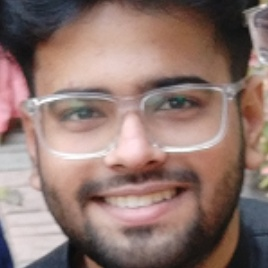
\includegraphics[height=.15\textwidth]{../imgs/saubhagya (28).jpg}
        \\
        \hline
        2                      & Avishkar      & 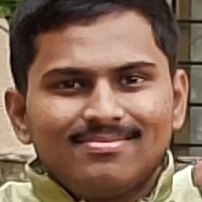
\includegraphics[height=.15\textwidth]{../imgs/avishkar (1).jpg}
        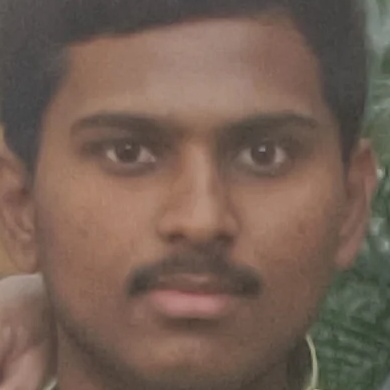
\includegraphics[height=.15\textwidth]{../imgs/avishkar (8).jpg}
        \\
        \hline
        3                      & Karad         & 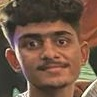
\includegraphics[height=.15\textwidth]{../imgs/sourab.jpg}
        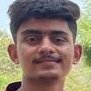
\includegraphics[height=.15\textwidth]{../imgs/sourab (12).jpg}
        \\
        \hline
        4                      & Krish         & 
\includegraphics[height=.15\textwidth]{../imgs/krish (4).jpg}
        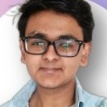
\includegraphics[height=.15\textwidth]{../imgs/krish (66).jpg}
        \\
        \hline
        5                      & Parth         & 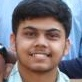
\includegraphics[height=.15\textwidth]{../imgs/parth (1).jpg}
        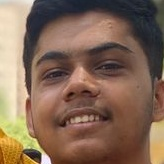
\includegraphics[height=.15\textwidth]{../imgs/parth (31).jpg}
        \\
        \hline
        6                      & Abhijeet         & 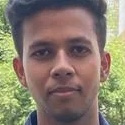
\includegraphics[height=.15\textwidth]{../imgs/abhijeet (3).jpg}
        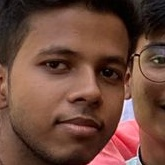
\includegraphics[height=.15\textwidth]{../imgs/abhijeet (5).jpg}
        \\
        \hline
        7                      & Naman         & 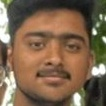
\includegraphics[height=.15\textwidth]{../imgs/naman (42).jpg}
        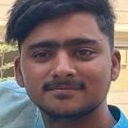
\includegraphics[height=.15\textwidth]{../imgs/naman (8).jpg}
        \\
        \hline
        8                      & Mayur         & 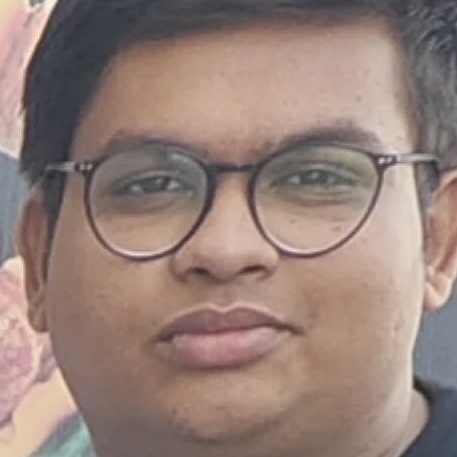
\includegraphics[height=.15\textwidth]{../imgs/mayur (13).jpg}
        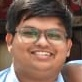
\includegraphics[height=.15\textwidth]{../imgs/mayur (1).jpg}
        \\
        \hline
    \end{tabular}
    \caption{Training Data Images}
\end{table}

\begin{table}[H]
    \centering
    \begin{tabular}{|c|c|c|}
        \hline
        \textbf{Serial Number} & \textbf{Name} & \textbf{Image}                                        \\
        \hline
        9                      & Sahaj         & 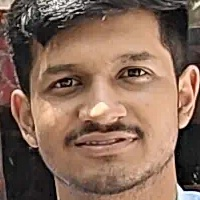
\includegraphics[height=.15\textwidth]{../imgs/sahaj (17).jpg}
        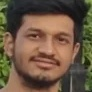
\includegraphics[height=.15\textwidth]{../imgs/sahaj (42).jpg}
        \\
        \hline
        10                      & Maitreyee         & 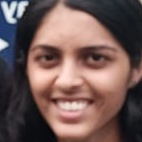
\includegraphics[height=.15\textwidth]{../imgs/maitreyee (21).jpg}
        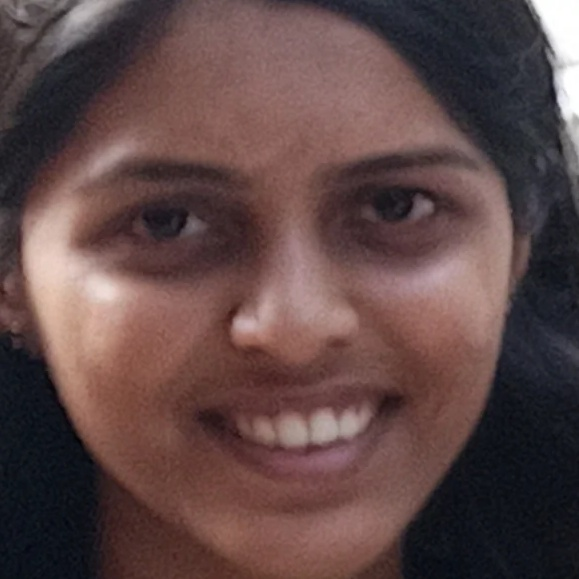
\includegraphics[height=.15\textwidth]{../imgs/maitreyee (78).jpg}
        \\
        \hline
        \hline
        11                      & Prathamesh         & 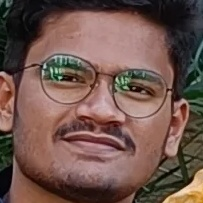
\includegraphics[height=.15\textwidth]{../imgs/prathamesh (27).jpg}
        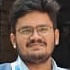
\includegraphics[height=.15\textwidth]{../imgs/prathamesh.jpg}
        \\
        \hline
        12                      & Khare         & 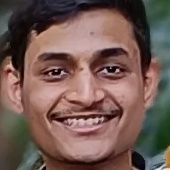
\includegraphics[height=.15\textwidth]{../imgs/khare.jpg}
        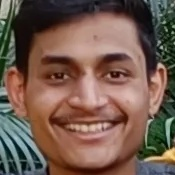
\includegraphics[height=.15\textwidth]{../imgs/khare (32).jpg}
        \\
        \hline
    \end{tabular}
    \caption{Training Data Images (Continued)}
\end{table}

\subsection{Creation of Dataset}
\subsubsection{Cropped Faces using openCV-haar-cascades}
The following code generated 18,832 possible faces (245x245px) each. The code uses the OpenCV library to detect faces in images and crop them. The cropped faces are then saved in a specified output folder. The code uses the Haar Cascade classifier for face detection, which is a popular method for real-time face detection. 
\begin{lstlisting}[language=Python]
import cv2
import os
import numpy as np

def detect_and_crop_faces(input_folder, output_folder, padding=10):
    if not os.path.exists(output_folder):
        os.makedirs(output_folder)
    
    face_cascade = cv2.CascadeClassifier(cv2.data.haarcascades + 'haarcascade_frontalface_default.xml')
    
    for filename in os.listdir(input_folder):
        if filename.lower().endswith(('png', 'jpg', 'jpeg', 'webp')):
            image_path = os.path.join(input_folder, filename)
            image = cv2.imread(image_path)
            
            if image is None:
                continue
            
            gray = cv2.cvtColor(image, cv2.COLOR_BGR2GRAY)
            faces = face_cascade.detectMultiScale(gray, scaleFactor=1.1, minNeighbors=5, minSize=(30, 30))
            
            for i, (x, y, w, h) in enumerate(faces):
                x1 = max(x - padding, 0)
                y1 = max(y - padding, 0)
                x2 = min(x + w + padding, image.shape[1])
                y2 = min(y + h + padding, image.shape[0])
                
                face_crop = image[y1:y2, x1:x2]
                output_path = os.path.join(output_folder, f"{os.path.splitext(filename)[0]}_face_{i}.jpg")
                cv2.imwrite(output_path, face_crop)
                print(f"Saved cropped face: {output_path}")

input_folder = os.path.join(os.getcwd(), "input_images")  
output_folder = os.path.join(os.getcwd(), "output_images") 

detect_and_crop_faces(input_folder, output_folder)
    
\end{lstlisting}
\textbf{Results of the above code are shown in the figure below. The images are cropped and saved in the output folder.}

\begin{figure}[H]
    \centering
    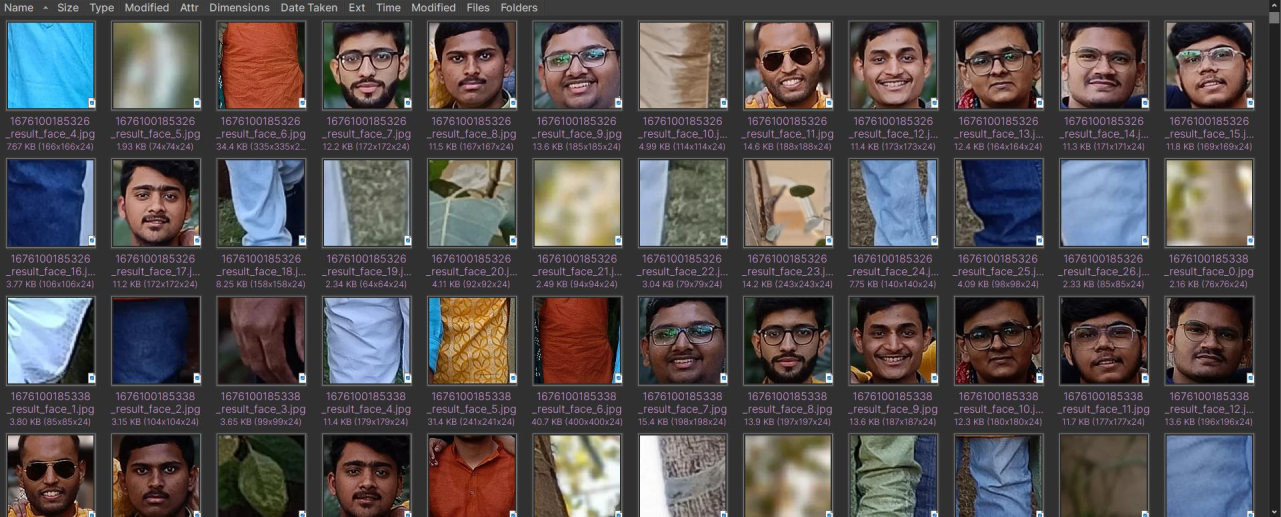
\includegraphics[width=.95\textwidth]{../imgs/Cropped images.png}
    \caption{Cropped Faces using OpenCV Haar Cascades}
\end{figure}

\begin{figure}[H]
    \centering
    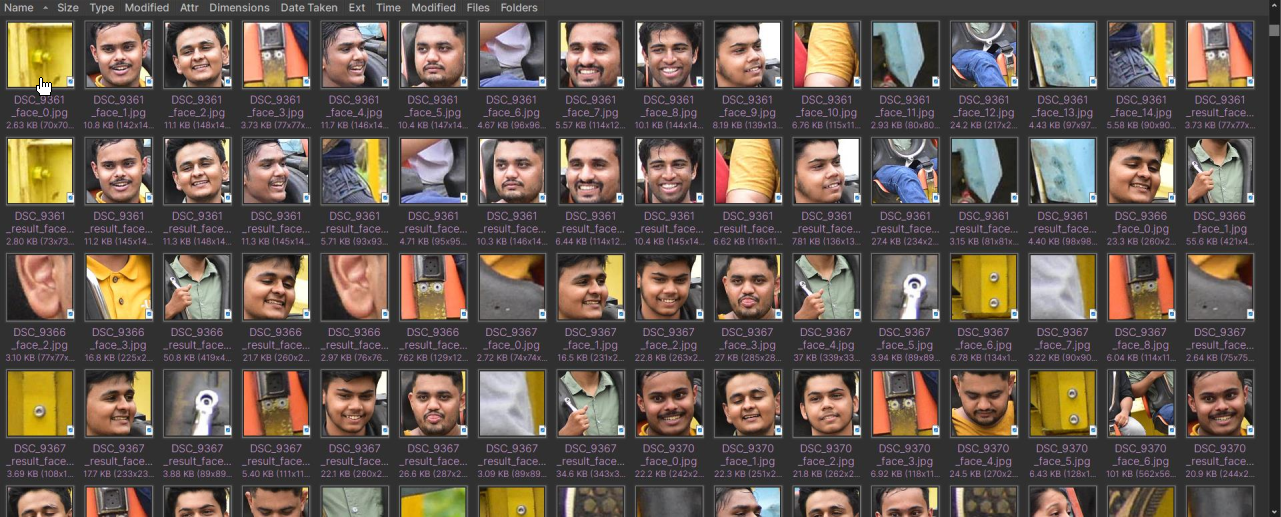
\includegraphics[width=.95\textwidth]{../imgs/Copped images 2.png}
    \caption{Cropped Faces using OpenCV Haar Cascades}
\end{figure}

\begin{figure}[H]
    \centering
    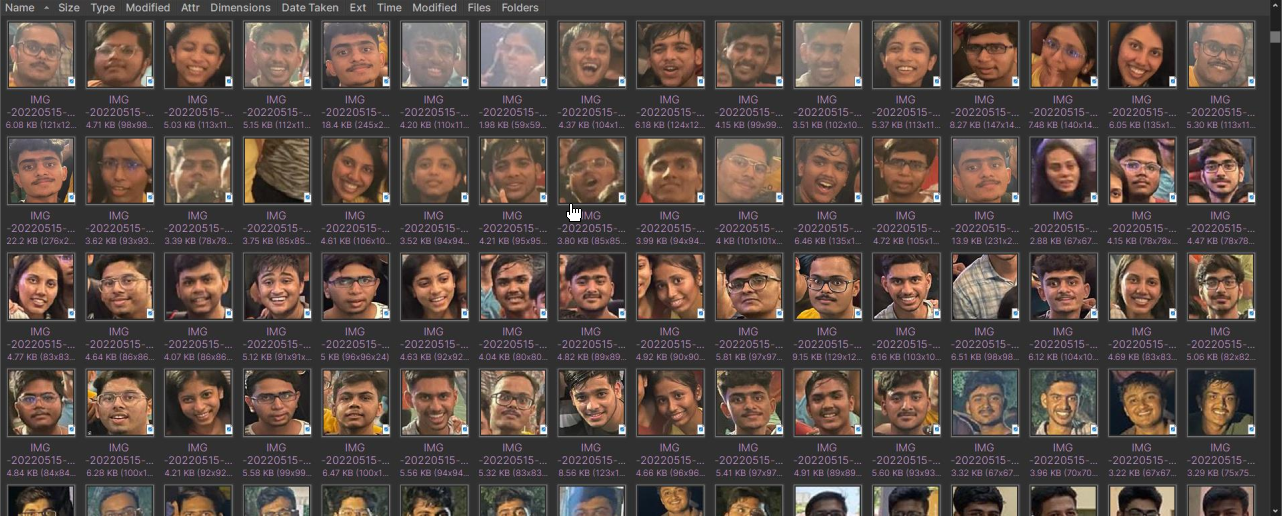
\includegraphics[width=.95\textwidth]{../imgs/Copped images 3.png}
    \caption{Cropped Faces using OpenCV Haar Cascades}
\end{figure}

\section{API Endpoints}
\subsection{Attendance API Endpoints}
\begin{figure}[H]
    \centering
    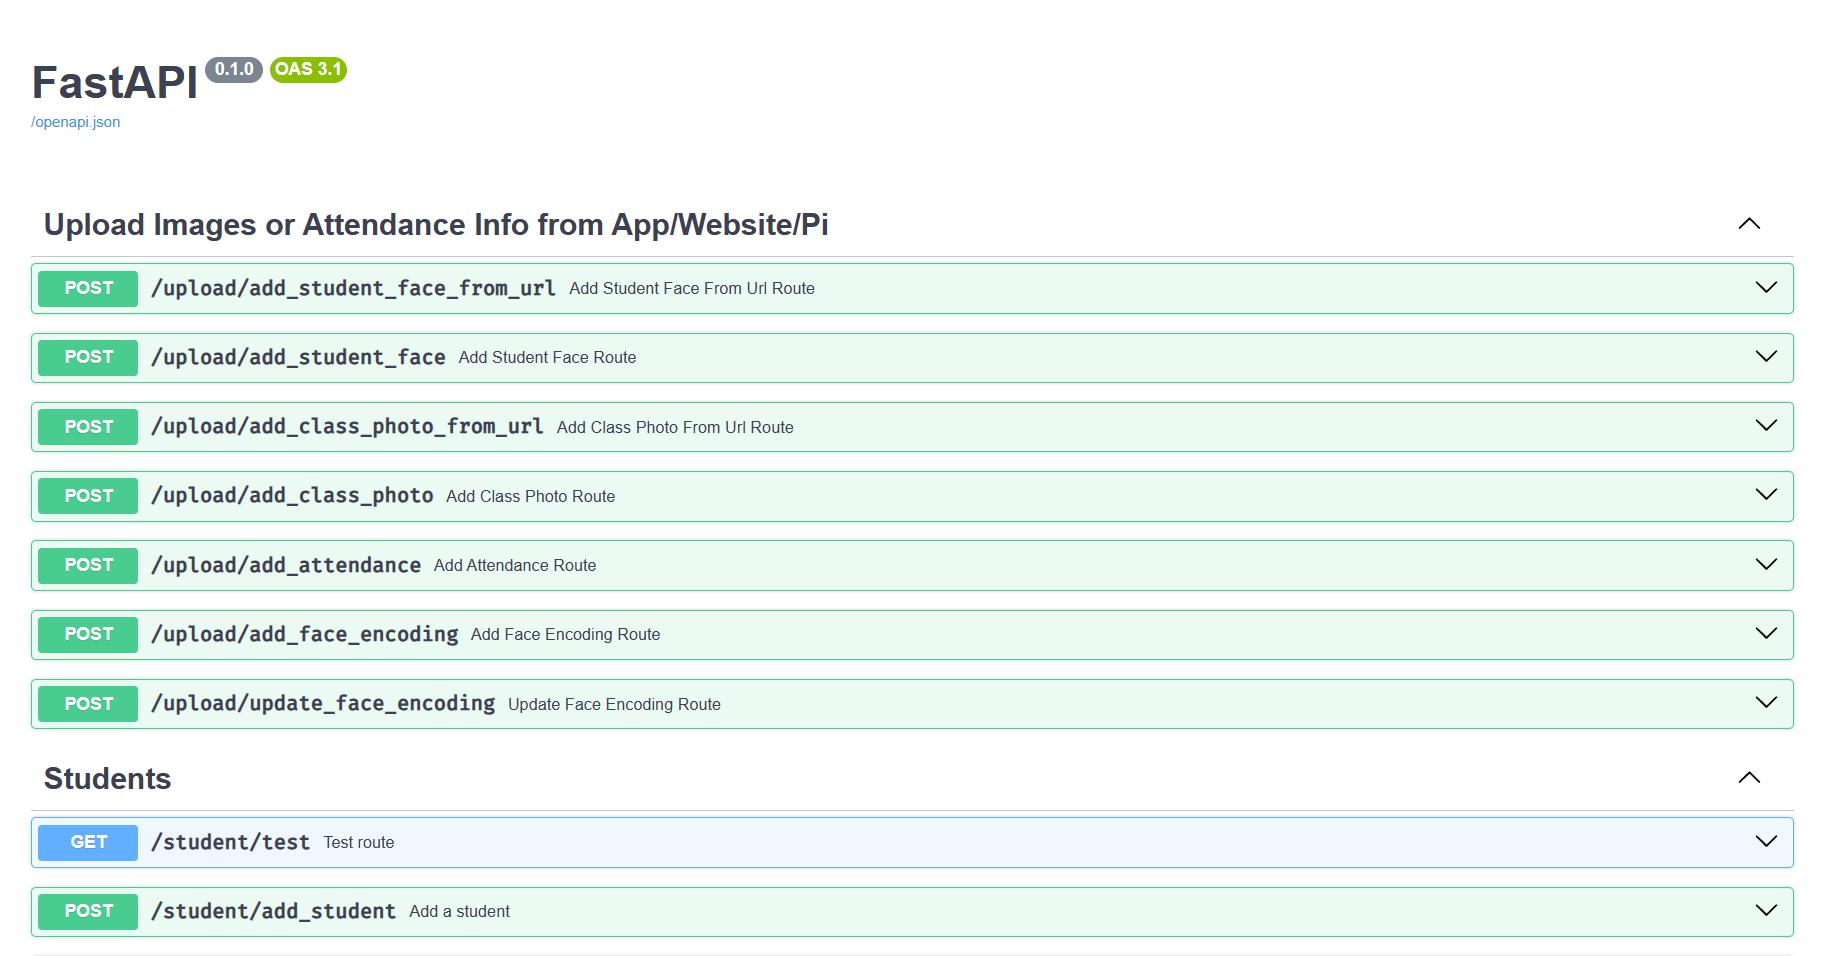
\includegraphics[width=.99\textwidth]{../imgs/swagger 1.jpg}
    \caption{API Endpoints for Attendance details}
\end{figure}

\subsection{Student API Endpoints}
\begin{figure}[H]
    \centering
    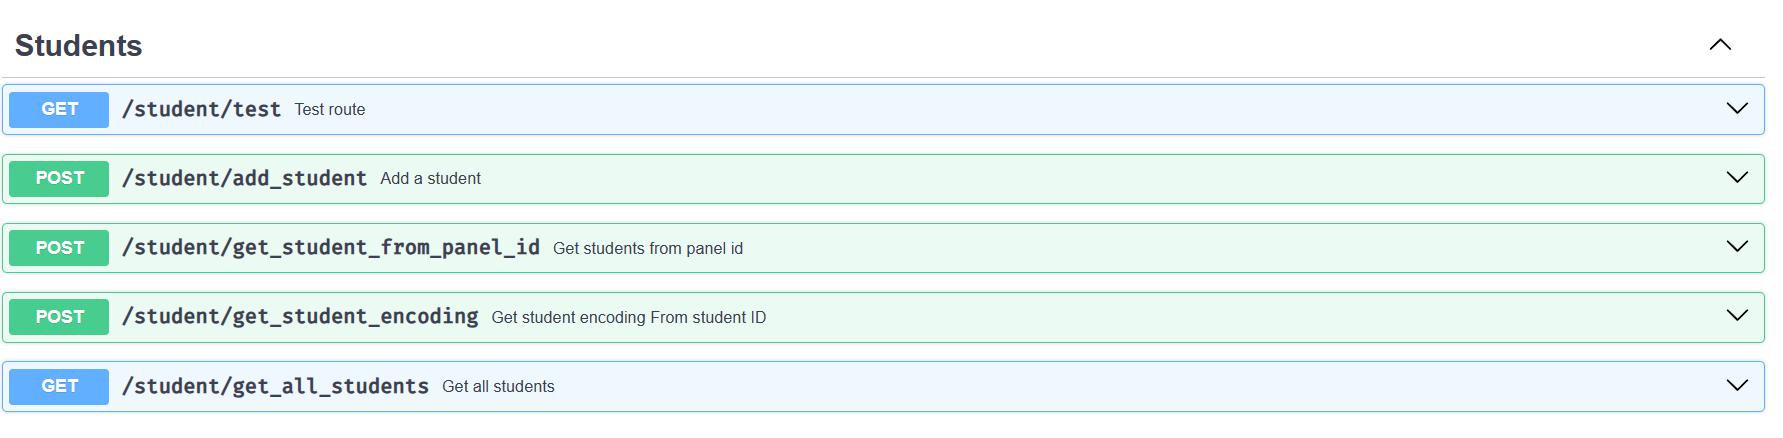
\includegraphics[width=.99\textwidth]{../imgs/swagger 2.jpg}
    \caption{API Endpoints for Student details}
\end{figure}

\subsection{Schools and Specialization API Endpoints}
\begin{figure}[H]
    \centering
    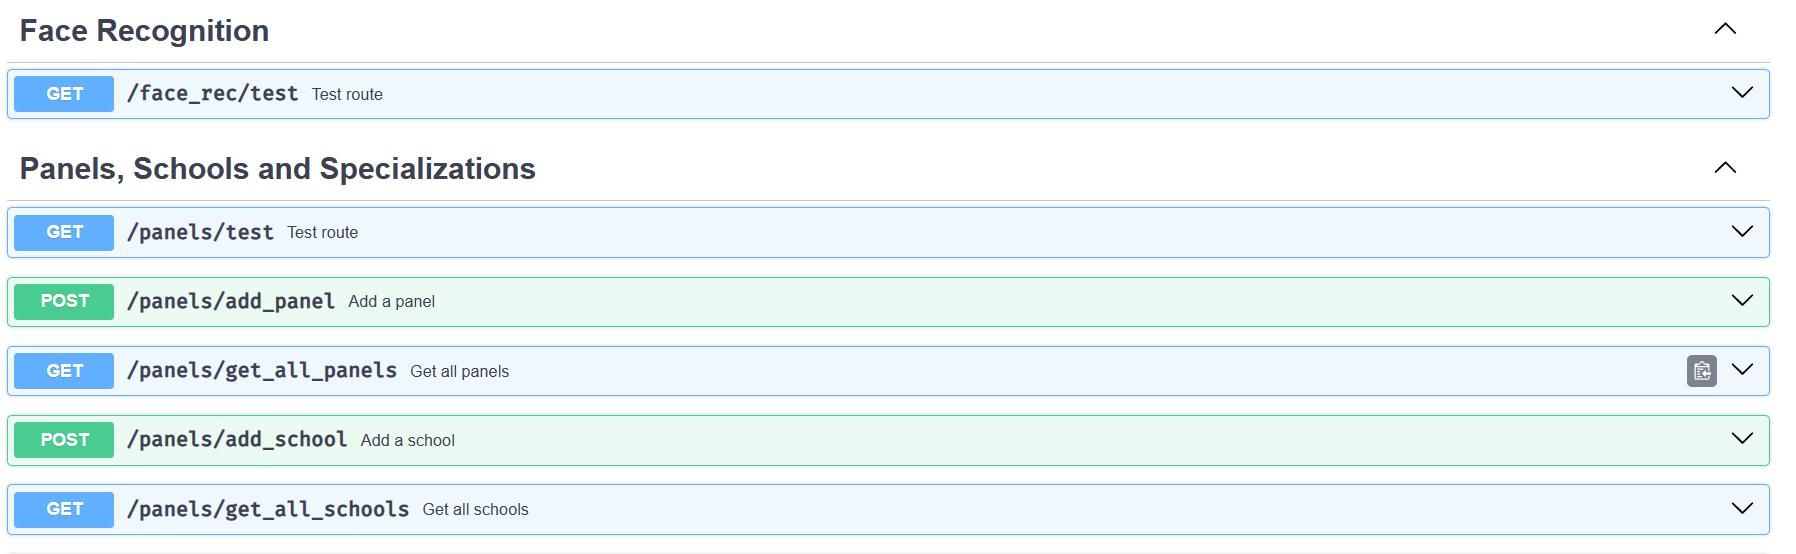
\includegraphics[width=.99\textwidth]{../imgs/swagger 3.jpg}
    \caption{API Endpoints for Schools and Specialization details}
\end{figure}

\subsection{Panel API Endpoints}
\begin{figure}[H]
    \centering
    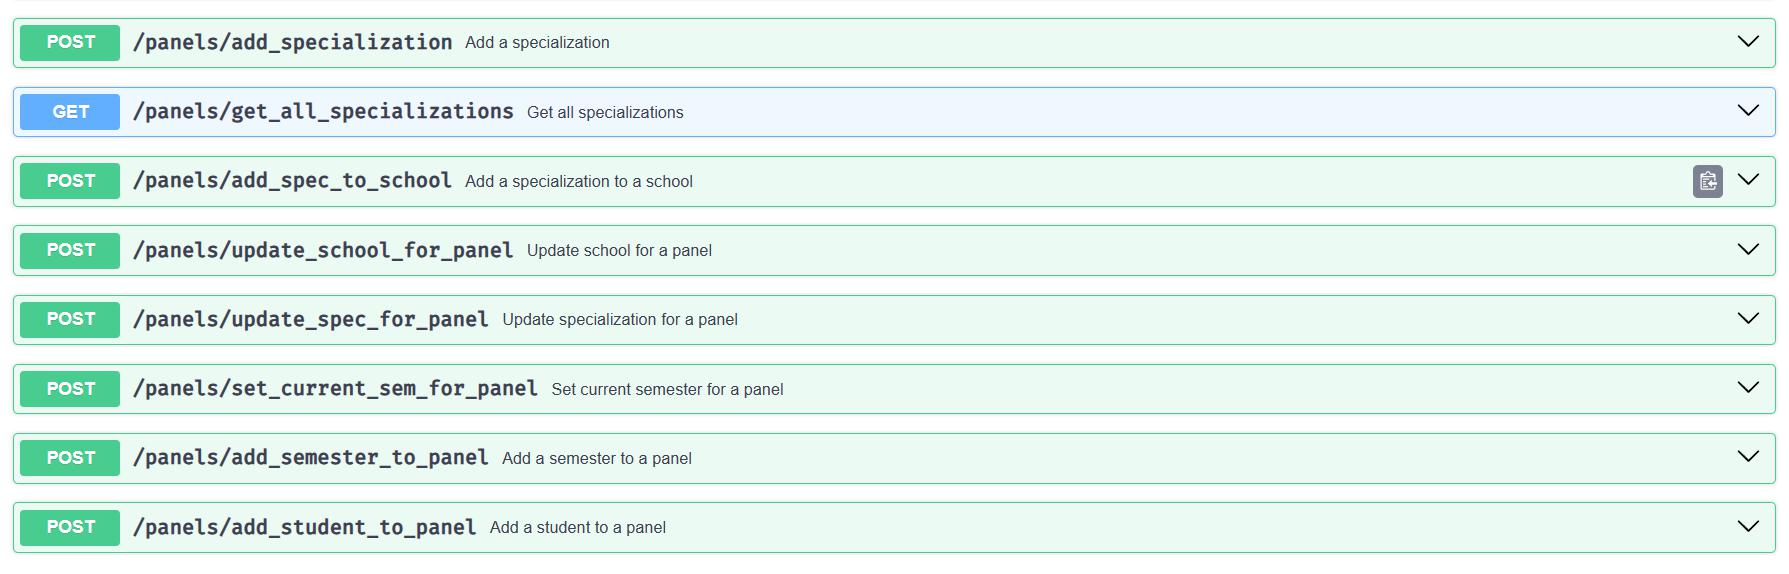
\includegraphics[width=.99\textwidth]{../imgs/swagger 4.jpg}
    \caption{API Endpoints for Panel details}
\end{figure}


\subsection{Rooms and Buildings API Endpoints}
\begin{figure}[H]
    \centering
    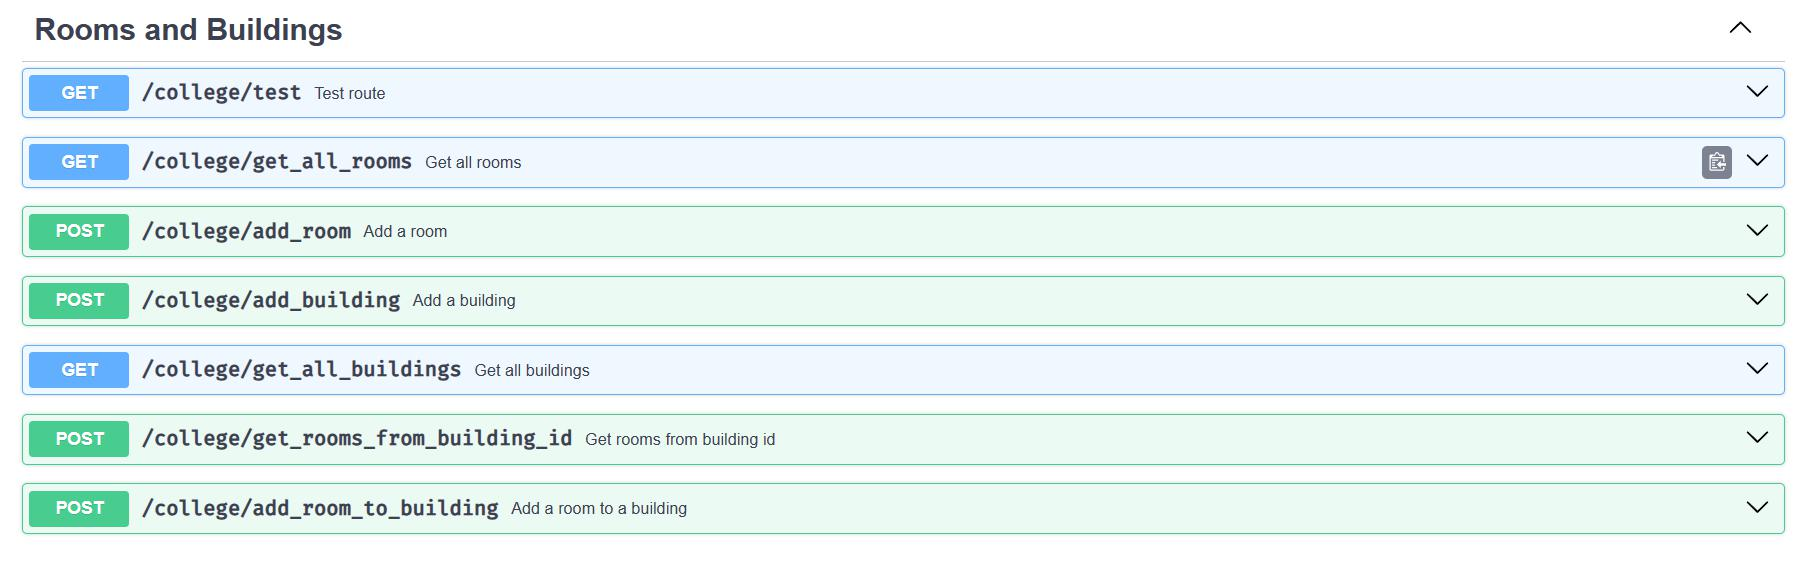
\includegraphics[width=.99\textwidth]{../imgs/swagger 5.jpg}
    \caption{API Endpoints for Rooms and Buildings details}
\end{figure}


\subsection{Subjects and Semesters API Endpoints}
\begin{figure}[H]
    \centering
    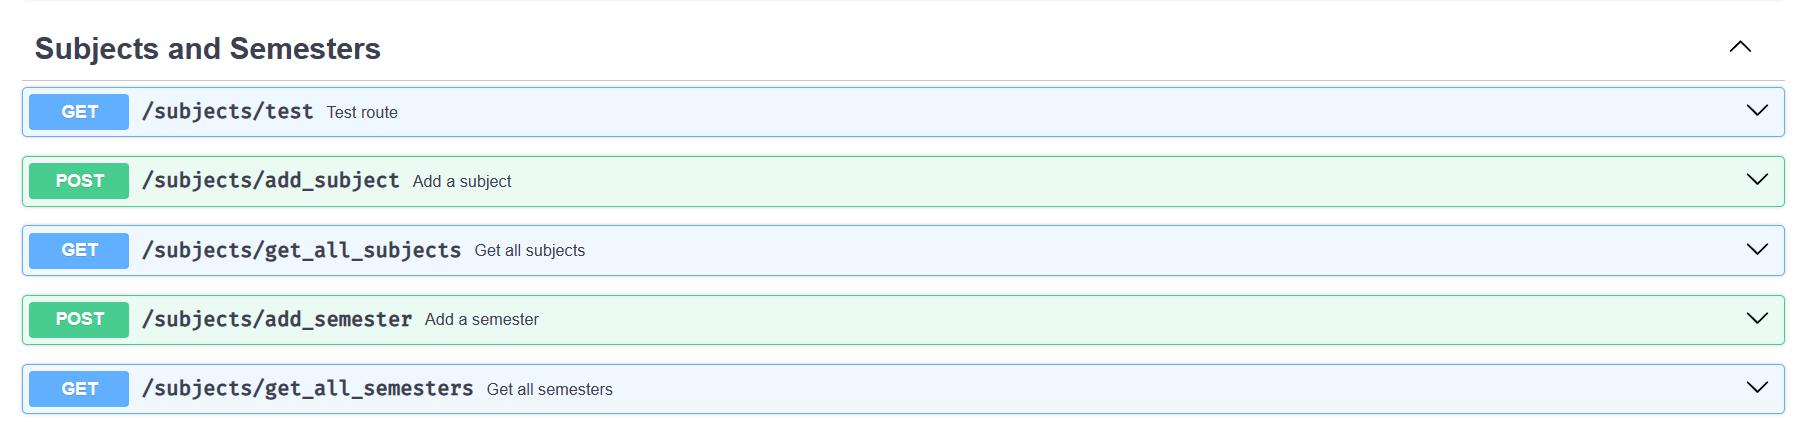
\includegraphics[width=.99\textwidth]{../imgs/swagger 6.jpg}
    \caption{API Endpoints for Subjects and Semesters details}
\end{figure}

\subsection{Teacher API Endpoints}
\begin{figure}[H]
    \centering
    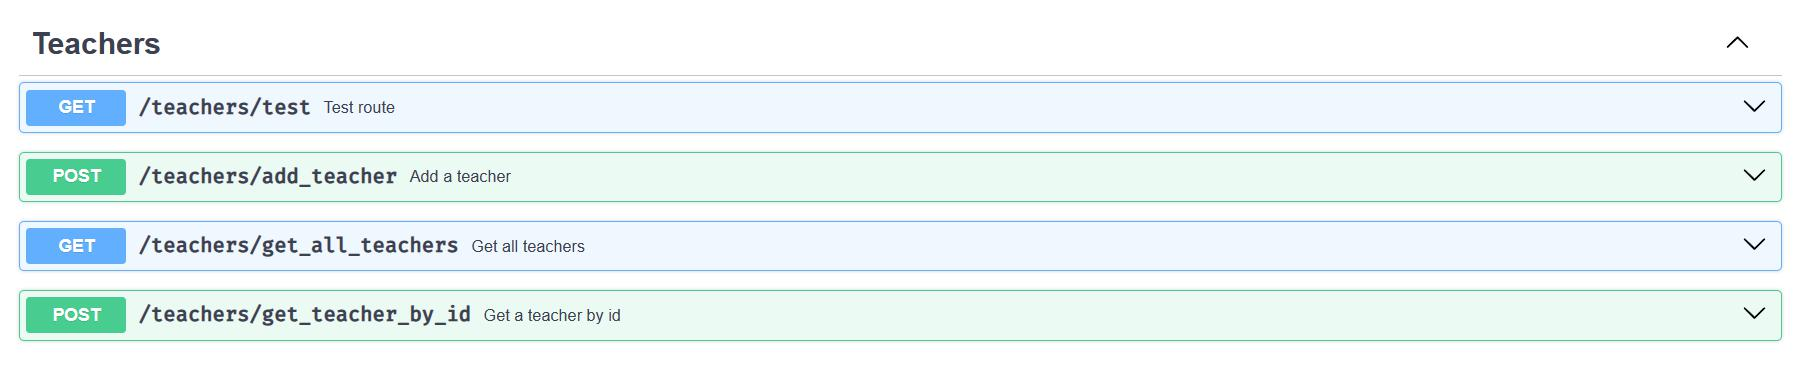
\includegraphics[width=.99\textwidth]{../imgs/swagger 7.jpg}
    \caption{API Endpoints for Teacher details}
\end{figure}

\subsection{Lecture API Endpoints}
\begin{figure}[H]
    \centering
    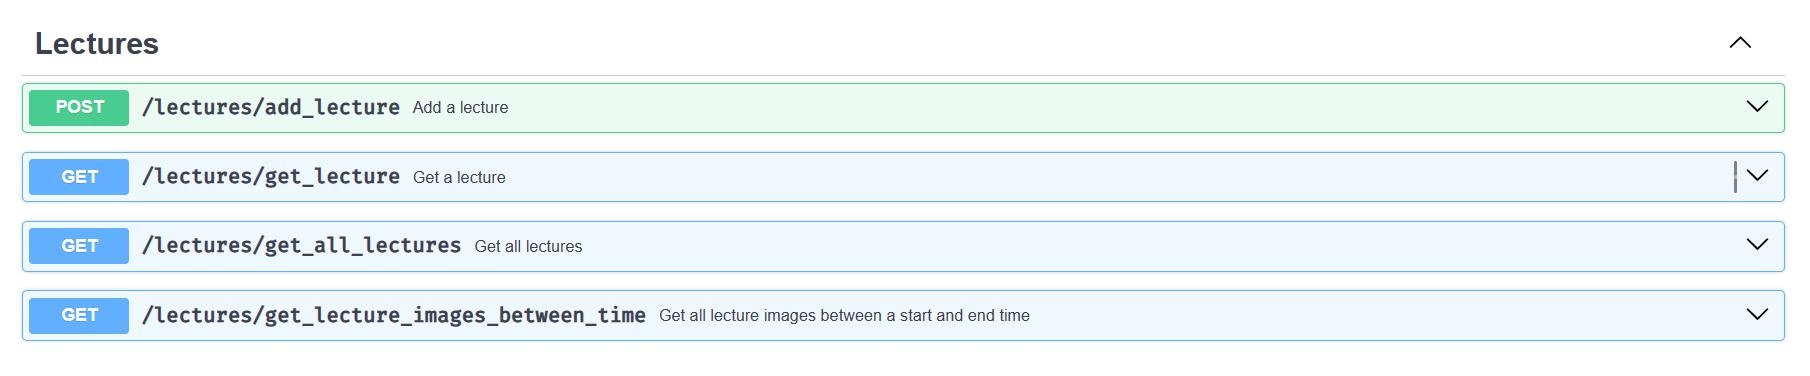
\includegraphics[width=.99\textwidth]{../imgs/swagger 8.jpg}
    \caption{API Endpoints for Lecture details}

\end{figure}

\section{Model Training}

\subsection{Code Snippet for face recognition using LBPH}
\begin{lstlisting}[language=Python]
import os
import cv2
import numpy as np
from sklearn.metrics import classification_report

base_path = "   "
image_size = (100, 100)

def load_images(folder, label, max_images=None):
    images = []
    labels = []
    for i, filename in enumerate(os.listdir(folder)):
        if max_images and i >= max_images:
            break
        img_path = os.path.join(folder, filename)
        img = cv2.imread(img_path, cv2.IMREAD_GRAYSCALE)
        if img is not None:
            img = cv2.resize(img, image_size)
            images.append(img)
            labels.append(label)
    return images, labels

def train_individual_models(base_path):
    person_dirs = [d for d in os.listdir(base_path) if os.path.isdir(os.path.join(base_path, d))]
    for person in person_dirs:
        print(f"\nTraining model for: {person}")
        
        # Positive samples (label = 1)
        pos_train_dir = os.path.join(base_path, person, 'train')
        pos_test_dir = os.path.join(base_path, person, 'test')
        pos_train_imgs, pos_train_labels = load_images(pos_train_dir, label=1)
        pos_test_imgs, pos_test_labels = load_images(pos_test_dir, label=1)

        # Negative samples (label = 0) from other people's train dirs
        neg_train_imgs = []
        neg_train_labels = []
        neg_test_imgs = []
        neg_test_labels = []
        for other_person in person_dirs:
            if other_person == person:
                continue
            other_train_dir = os.path.join(base_path, other_person, 'train')
            other_test_dir = os.path.join(base_path, other_person, 'test')
            imgs, labels = load_images(other_train_dir, label=0, max_images=len(pos_train_imgs)//(len(person_dirs)-1))
            neg_train_imgs += imgs
            neg_train_labels += labels
            imgs, labels = load_images(other_test_dir, label=0, max_images=len(pos_test_imgs)//(len(person_dirs)-1))
            neg_test_imgs += imgs
            neg_test_labels += labels

        # Combine positives and negatives
        X_train = pos_train_imgs + neg_train_imgs
        y_train = pos_train_labels + neg_train_labels
        X_test = pos_test_imgs + neg_test_imgs
        y_test = pos_test_labels + neg_test_labels

        # Train LBPH model
        model = cv2.face.LBPHFaceRecognizer_create()
        model.train(X_train, np.array(y_train))

        # Evaluate
        predictions = []
        for face in X_test:
            label_pred, _ = model.predict(face)
            predictions.append(label_pred)

        print(classification_report(y_test, predictions, target_names=["Other", person]))

train_individual_models(base_path)
\end{lstlisting}
\subsection{Code Snippet for face recognition using face\_net}
\begin{lstlisting}[language=Python]
import os
import torch
import numpy as np
from PIL import Image
from tqdm import tqdm
from torchvision import transforms
from facenet_pytorch import InceptionResnetV1, MTCNN
from sklearn.metrics.pairwise import cosine_similarity

# Device config
device = torch.device('cuda' if torch.cuda.is_available() else 'cpu')

# Load FaceNet model
model = InceptionResnetV1(pretrained='vggface2').eval().to(device)

# MTCNN for face detection
mtcnn = MTCNN(image_size=160, margin=0, min_face_size=20, keep_all=False, device=device)

# Define dataset path
dataset_path = 'comprehensive_db\\comprehensive_db'

# Function to extract embeddings
def get_embedding(img_path):
    img = Image.open(img_path).convert('RGB')
    face = mtcnn(img)
    if face is not None:
        face_embedding = model(face.unsqueeze(0).to(device))
        return face_embedding.detach().cpu().numpy()[0]
    else:
        return None

# Step 1: Prepare reference embeddings from training data
reference_embeddings = {}  # person -> list of embeddings

print("\nCreating reference embeddings from train data...")
for person in os.listdir(dataset_path):
    person_train_path = os.path.join(dataset_path, person, 'train')
    embeddings = []
    for img_name in os.listdir(person_train_path):
        img_path = os.path.join(person_train_path, img_name)
        emb = get_embedding(img_path)
        if emb is not None:
            embeddings.append(emb)
    if embeddings:
        reference_embeddings[person] = np.mean(embeddings, axis=0)  # Mean embedding

# Step 2: Evaluate on test data
print("\nEvaluating on test data...")
correct = 0
total = 0

for person in os.listdir(dataset_path):
    person_test_path = os.path.join(dataset_path, person, 'test')
    for img_name in os.listdir(person_test_path):
        img_path = os.path.join(person_test_path, img_name)
        test_emb = get_embedding(img_path)
        if test_emb is None:
            continue

        # Compare with reference embeddings
        similarities = {}
        for ref_person, ref_emb in reference_embeddings.items():
            sim = cosine_similarity([test_emb], [ref_emb])[0][0]
            similarities[ref_person] = sim

        predicted_person = max(similarities, key=similarities.get)
        if predicted_person == person:
            correct += 1
        total += 1

accuracy = correct / total if total > 0 else 0
print(f"\n FaceNet Recognition Accuracy: {accuracy:.2f} ({correct}/{total})")

\end{lstlisting}
\subsection{Code Snippet for face recognition using res\_net}
\begin{lstlisting}[language=Python]

from torchvision import models
from torch.utils.data import DataLoader
import torch.nn as nn
import torch
import torch.optim as optim

# Paths
train_data_path = 'comprehensive_db\\comprehensive_db'

# Transforms
transform = transforms.Compose([
    transforms.Resize((224, 224)),
    transforms.ToTensor(),
    transforms.Normalize([0.5]*3, [0.5]*3)
])

# Load dataset
train_dataset = FaceTrainDataset(train_data_path, transform=transform)
train_loader = DataLoader(train_dataset, batch_size=32, shuffle=True)

# Model setup
device = torch.device('cuda' if torch.cuda.is_available() else 'cpu')
model = models.resnet50(pretrained=True)

# Replace the classifier for num_classes
num_classes = len(train_dataset.class_to_idx)
model.fc = nn.Linear(model.fc.in_features, num_classes)
model.to(device)

# Loss and optimizer
criterion = nn.CrossEntropyLoss()
optimizer = optim.Adam(model.parameters(), lr=0.0001)

# Training loop
num_epochs = 5
for epoch in range(num_epochs):
    model.train()
    total_loss = 0
    correct = 0
    total = 0
    for images, labels in train_loader:
        images = images.to(device)
        labels = labels.to(device)

        outputs = model(images)
        loss = criterion(outputs, labels)
        optimizer.zero_grad()
        loss.backward()
        optimizer.step()

        total_loss += loss.item()
        _, predicted = torch.max(outputs, 1)
        correct += (predicted == labels).sum().item()
        total += labels.size(0)

    acc = 100 * correct / total
    print(f"Epoch [{epoch+1}/{num_epochs}] - Loss: {total_loss:.4f}, Accuracy: {acc:.2f}%")

# Save model
torch.save(model.state_dict(), "resnet50_face_recognizer.pth")
\end{lstlisting}

\chapter{Performance Evaluation and Testing}
\section{Evaluation Metrics}

\begin{enumerate}
    \item Accuracy: The percentage of correctly identified faces out of the total number of faces.
    \item Precision: The percentage of correctly identified faces out of the total number of faces identified.
    \item Recall: The percentage of correctly identified faces out of the total number of faces in the dataset.
    \item F1 Score: The harmonic mean of precision and recall, which provides a balanced measure of accuracy.
\end{enumerate}


\section{Testing Methodology}
\begin{enumerate}
    \item Dataset Preparation: The dataset was divided into training and testing sets, with 80\% of the images used for training and 20\% for testing.
    \item Model Training: The face recognition model was trained using the training set, and the parameters were optimized for better accuracy.
    \item Model Testing: The trained model was tested using the testing set, and the evaluation metrics were calculated based on the results.
    \item Performance Comparison: The performance of different face recognition algorithms was compared based on the evaluation metrics.
\end{enumerate}

\section{Testing and Training Dataset}


\subsubsection{Manually Segregated photos for 5 people and labelled them}
\begin{figure}[H]
    \centering
    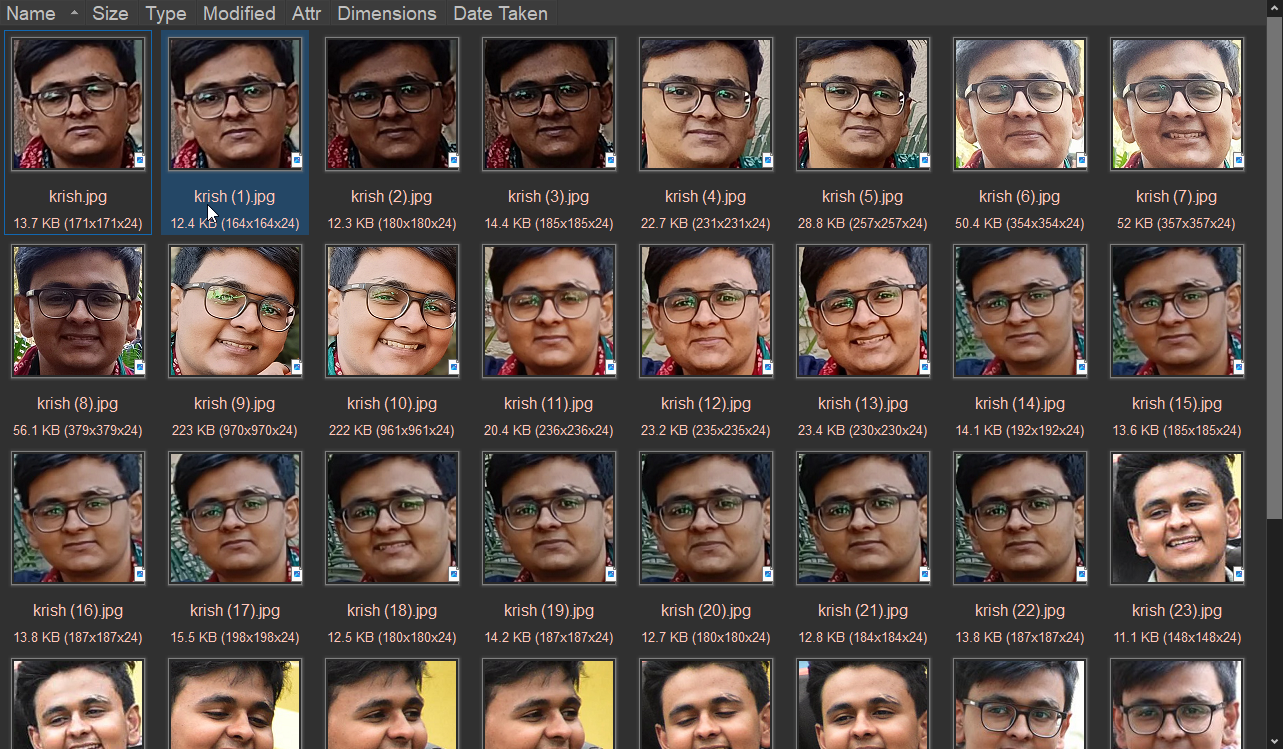
\includegraphics[width=.95\textwidth]{../imgs/krishnaraj.png}
    \caption{Krishnaraj's Segregated Images}
\end{figure}
\begin{figure}[H]
    \centering
    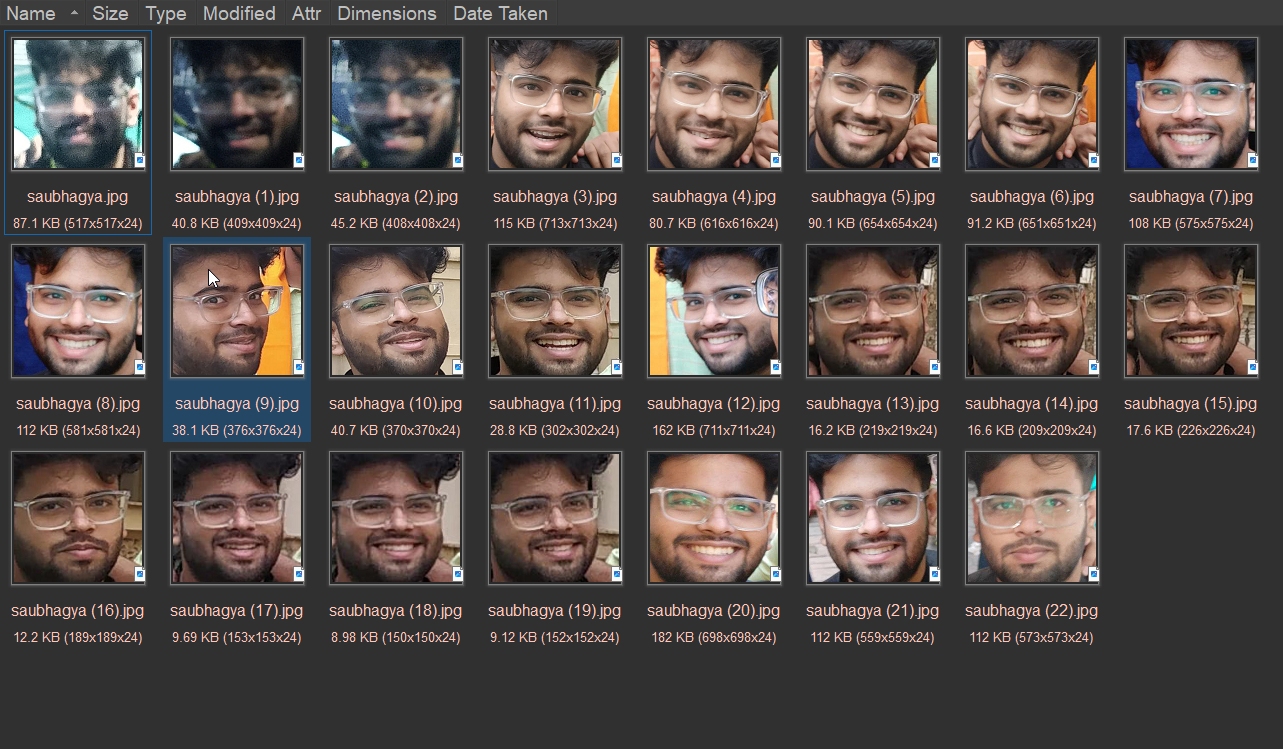
\includegraphics[width=.95\textwidth]{../imgs/saubhagya.png}
    \caption{Saubhagya's Segregated Images}
\end{figure}
\begin{figure}[H]
    \centering
    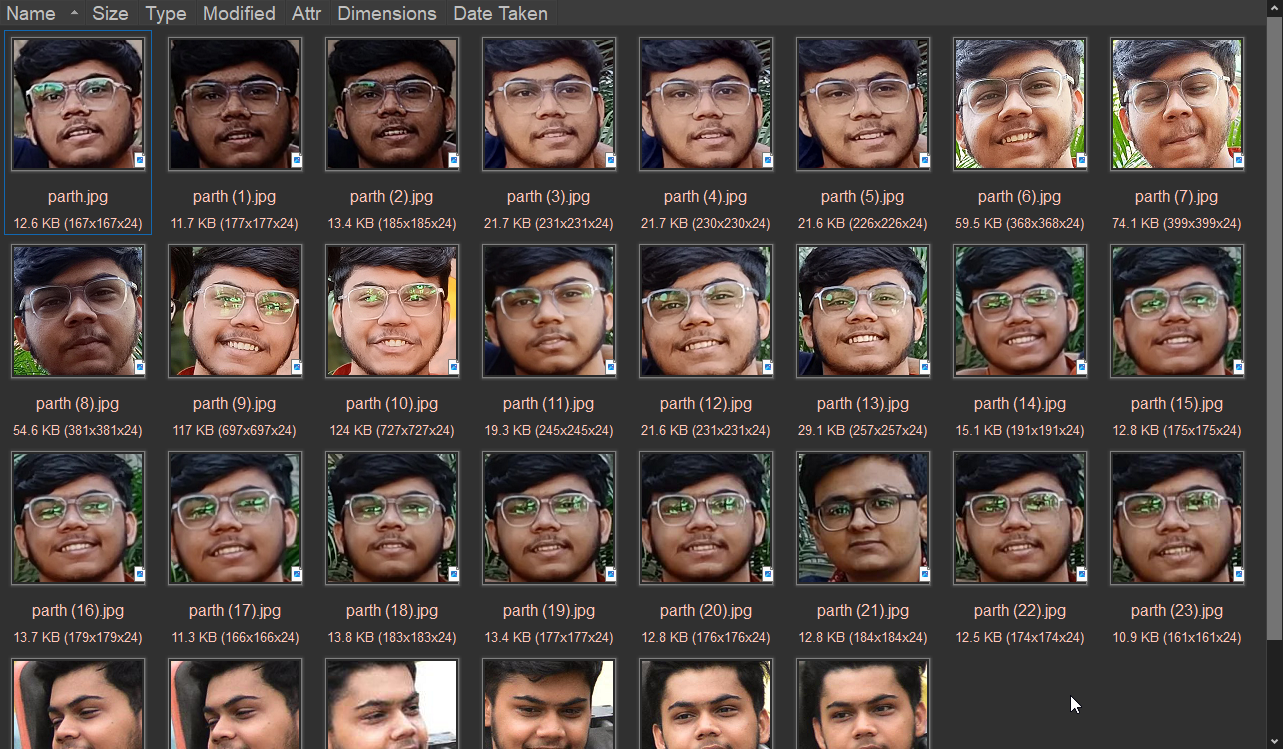
\includegraphics[width=.95\textwidth]{../imgs/parth.png}
    \caption{Parth's Segregated Images}
\end{figure}

\begin{figure}[H]
    \centering
    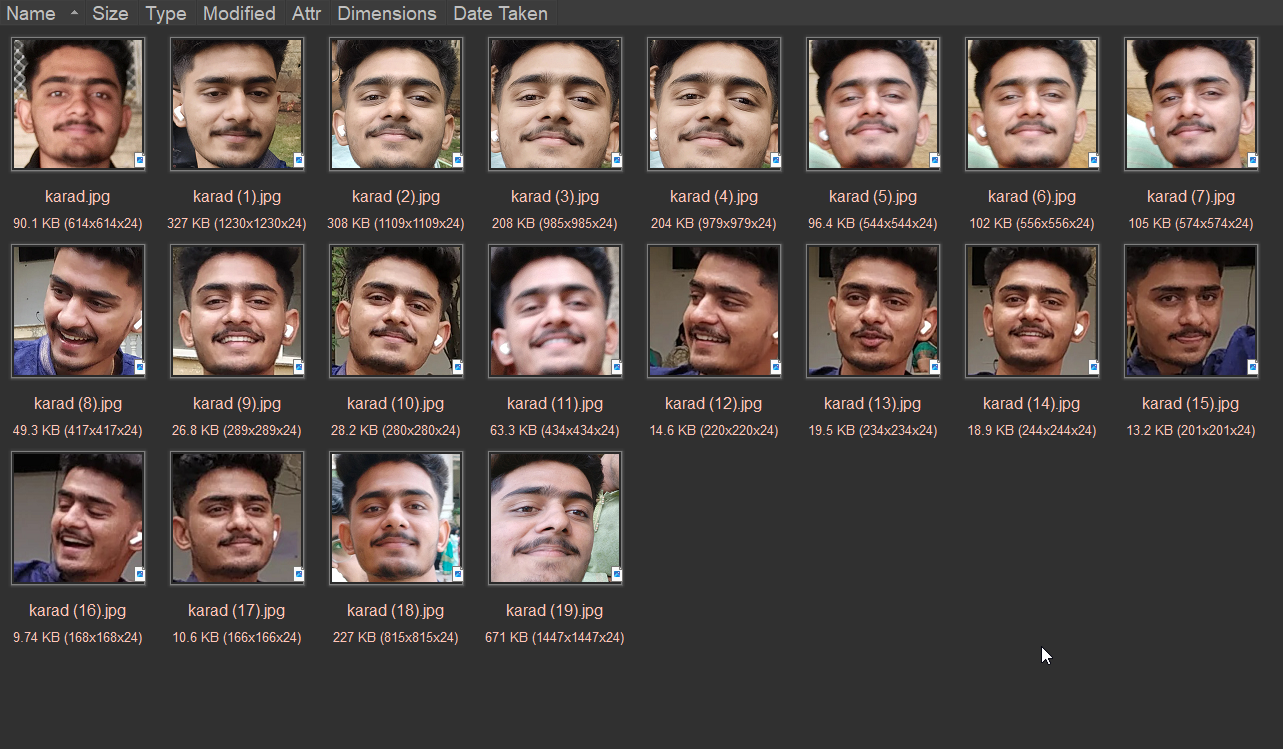
\includegraphics[width=.95\textwidth]{../imgs/sourab.png}
    \caption{Sourab's Segregated Images}
\end{figure}

\begin{figure}[H]
    \centering
    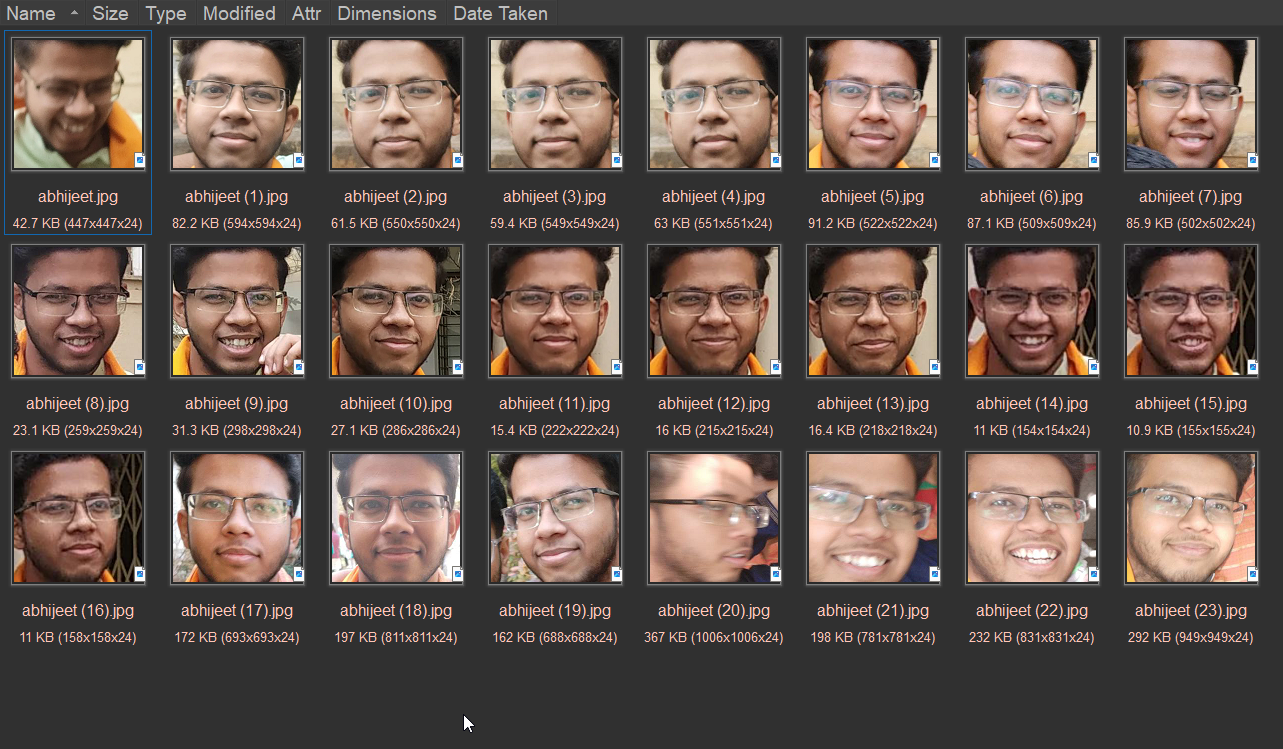
\includegraphics[width=.95\textwidth]{../imgs/abhijeet.png}
    \caption{Abhijeet's Segregated Images}
\end{figure}

\chapter{Deployment Strategies}

\section{Deployment Environment}
\begin{itemize}
    \item The application is designed to be deployed on a cloud-based server, ensuring scalability and accessibility.
    \item The backend is built using FastAPI, which allows for efficient handling of requests and responses.
    \item The database is managed using MongoDB, providing a flexible and scalable solution for data storage.
    \item The frontend is developed using Flutter, enabling cross-platform compatibility for both Android and iOS devices.
    \item The application can be deployed on platforms like AWS, Google Cloud, or Azure, ensuring high availability and reliability.
\end{itemize}

\section{Deployment Steps}
\begin{enumerate}
    \item Set up a cloud-based server with the required specifications (CPU, RAM, storage).
    \item Install the necessary software dependencies (Python, FastAPI, MongoDB, Flutter).
    \item Deploy the backend API using FastAPI and connect it to the MongoDB database.
    \item Build and deploy the Flutter application for both Android and iOS platforms.
    \item Configure domain and SSL certificates for secure access to the application.
    \item Test the application in the deployed environment to ensure functionality and performance.
    
    \item Monitor the application for any issues and optimize performance as needed.
\end{enumerate}

\section{Deployment Challenges}
\begin{itemize}
    \item Ensuring compatibility across different platforms and devices can be challenging, especially with Flutter.
    \item Managing database connections and ensuring data integrity during high traffic periods.
    \item Handling security concerns related to user data and ensuring compliance with data protection regulations.
    \item Optimizing the performance of the application to handle a large number of concurrent users.
    \item Ensuring proper documentation and support for users to facilitate smooth onboarding and usage of the application.
    
\end{itemize}

\section{Security Concerns}
\begin{itemize}
    \item Implementing secure authentication mechanisms to protect user data and prevent unauthorized access.
    \item Encrypting sensitive data stored in the database to ensure data privacy and security.
    \item Regularly updating the application and its dependencies to patch any security vulnerabilities.
    \item Monitoring the application for any suspicious activities and implementing intrusion detection systems.
    \item Educating users about best practices for data security and privacy when using the application.
\end{itemize}

\chapter{Result and Analysis}
\section{Model 1: LBPH Face Recognizer}
\subsection{Confusion Metrics}

\begin{figure}[H]
    \centering
    \begin{minipage}{0.48\textwidth}
        \centering
        \begin{tabular}{|c|c|}
            \hline
            \textbf{Metric} & \textbf{Value} \\ 
            \hline
            Accuracy        & 70\%           \\ 
            \hline
            Precision       & 85\%           \\ 
            \hline
            Recall          & 71\%           \\ 
            \hline
            F1 Score        & 73\%         \\ 
            \hline
        \end{tabular}
        \caption{Confusion Matrix of LBPH Face Recognizer}
        \label{tab:confusion-metrics}
    \end{minipage}
    \hfill
    \begin{minipage}{0.48\textwidth}
        \centering
        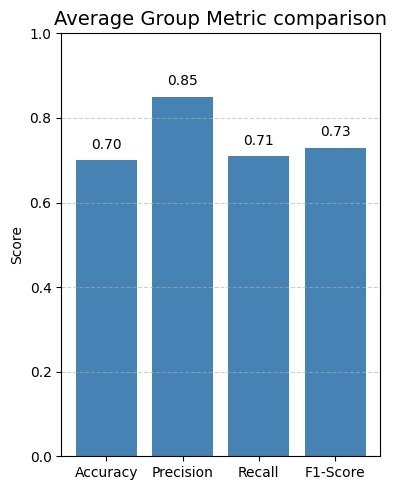
\includegraphics[width=\textwidth]{../imgs/model_1_cm.jpg}
        \caption{Accuracy per Person (Class) - LBPH Face Recognizer}
        \label{fig:confusion-matrix}
    \end{minipage}
\end{figure}

\subsection{Per Person Results}
Graphs showing the accuracy of each person in the dataset. The results indicate that the model performs well for most individuals, with some variations in accuracy based on the number of images available for training.
\begin{figure}[H]
    \centering
    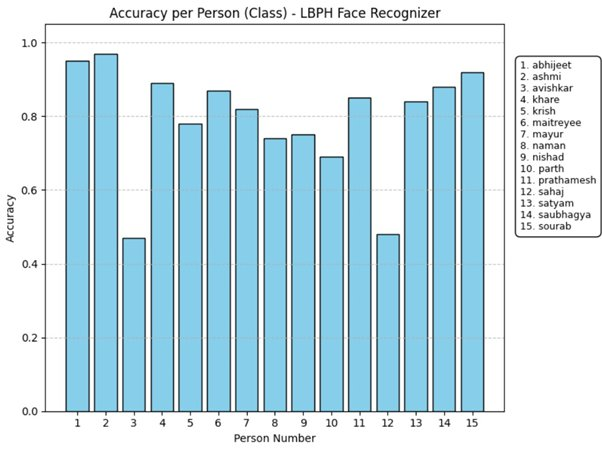
\includegraphics[width=.95\textwidth]{../imgs/model_1_per_person.jpg}
    \caption{Accuracy per Person (Class) - LBPH Face Recognizer}
\end{figure}

\section{Model 2: Facenet Face Recognizer}
\subsection{Confusion Metrics}

\begin{figure}[H]
    \centering
    \begin{minipage}{0.48\textwidth}
        \centering
        \begin{tabular}{|c|c|}
            \hline
            \textbf{Metric} & \textbf{Value} \\ 
            \hline
            Accuracy        & 87.63\%           \\ 
            \hline
            Precision       & 81.63\%           \\ 
            \hline
            Recall          & 84.63\%           \\ 
            \hline
            F1 Score        & 82.63\%         \\ 
            \hline
        \end{tabular}
        \caption{Confusion Matrix of Facenet Face Recognizer}
        \label{tab:confusion-metrics}
    \end{minipage}
    \hfill
    \begin{minipage}{0.48\textwidth}
        \centering
        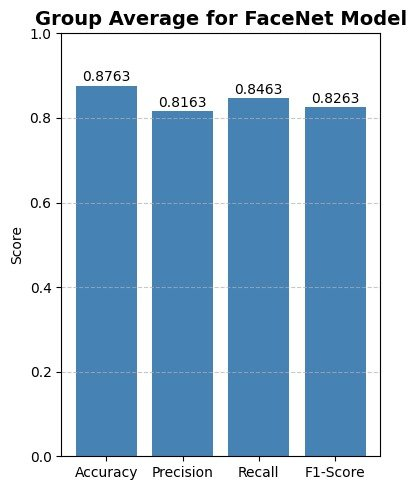
\includegraphics[width=\textwidth]{../imgs/model_2_cm (1).jpg}
        \caption{Accuracy per Person (Class) - Facenet Face Recognizer}
        \label{fig:confusion-matrix}
    \end{minipage}
\end{figure}

\subsection{Per Person Results}
Graphs showing the accuracy of each person in the dataset. The results indicate that the model performs well for most individuals, with some variations in accuracy based on the number of images available for training.
\begin{figure}[H]
    \centering
    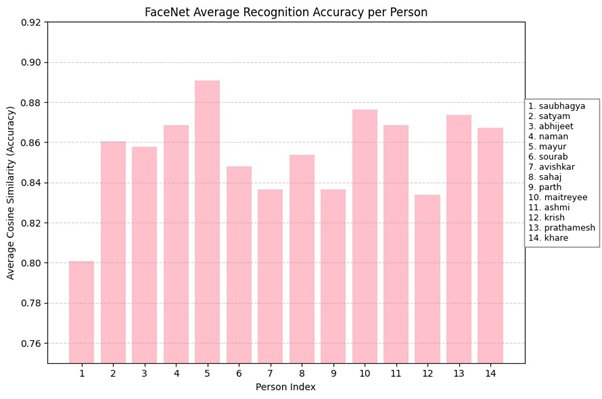
\includegraphics[width=.95\textwidth]{../imgs/model_2_per_person.jpg}
    \caption{Accuracy per Person (Class) - Facenet Face Recognizer}
\end{figure}

\section{Model 3: Resnet Face Recognizer}
\subsection{Confusion Metrics}

\begin{figure}[H]
    \centering
    \begin{minipage}{0.48\textwidth}
        \centering
        \begin{tabular}{|c|c|}
            \hline
            \textbf{Metric} & \textbf{Value} \\ 
            \hline
            Accuracy        & 91.44\%           \\ 
            \hline
            Precision       & 88.73\%           \\ 
            \hline
            Recall          & 91.48\%           \\ 
            \hline
            F1 Score        & 89.32\%         \\ 
            \hline
        \end{tabular}
        \caption{Confusion Matrix of Resnet Face Recognizer}
        \label{tab:confusion-metrics}
    \end{minipage}
    \hfill
    \begin{minipage}{0.48\textwidth}
        \centering
        \includegraphics[width=\textwidth]{../imgs/model_3_cp.jpg}
        \caption{Accuracy per Person (Class) - Resnet Face Recognizer}
        \label{fig:confusion-matrix}
    \end{minipage}
\end{figure}

\subsection{Per Person Results}
Graphs showing the accuracy of each person in the dataset. The results indicate that the model performs well for most individuals, with some variations in accuracy based on the number of images available for training.
\begin{figure}[H]
    \centering
    \includegraphics[width=.95\textwidth]{../imgs/model_3_per_person.jpg}
    \caption{Accuracy per Person (Class) - Resnet Face Recognizer}
\end{figure}

\section{Final Comparison} 
Resnet Face Recognizer outperformed the other two models in terms of accuracy, precision, recall, and F1 score. The results indicate that Resnet is the most effective model for face recognition tasks in this dataset.
\begin{figure}[H]
    \centering
    \includegraphics[width=.95\textwidth]{../imgs/final_model_comp.jpg}
    \caption{Final Model Comparison}
\end{figure}
\chapter{Applications}

\section{Educational Institutions}
\begin{itemize}
    \item \textbf{Automated Attendance Tracking:} The app can be used in schools, colleges, and universities to automate attendance marking, reducing manual errors and saving time.
    \item \textbf{Classroom Analytics:} Provides insights into Lectures attendance trends, helping educators identify patterns of absenteeism and take corrective actions.
    \item \textbf{Examination Monitoring:} Ensures only authorized students are present during exams by verifying their identity through facial recognition.
\end{itemize}

\section{Corporate Environments}
\begin{itemize}
    \item \textbf{Employee Time Tracking:} Automates attendance logging for employees, integrating seamlessly with HR systems for payroll and performance evaluation.
    \item \textbf{Access Control:} Restricts access to secure areas within office premises by verifying employee identities.
    \item \textbf{Remote Work Monitoring:} Tracks attendance for remote employees during virtual meetings or work-from-home scenarios.
\end{itemize}

\section{Healthcare Facilities}
\begin{itemize}
    \item \textbf{Patient Identification:} Ensures accurate identification of patients during check-ins, reducing errors in medical records.
    \item \textbf{Staff Attendance:} Tracks attendance of healthcare workers, ensuring adequate staffing levels at all times.
    \item \textbf{Visitor Management:} Monitors and records visitor entries for enhanced security in hospitals and clinics.
\end{itemize}

\section{Government and Public Sector}
\begin{itemize}
    \item \textbf{Public Office Attendance:} Tracks attendance of government employees, ensuring accountability and transparency.
    \item \textbf{Voter Verification:} Can be used during elections to verify voter identities and prevent fraud.
    \item \textbf{Public Safety:} Enhances security in public spaces by identifying individuals in real-time.
\end{itemize}

\section{Retail and Hospitality}
\begin{itemize}
    \item \textbf{Customer Personalization:} Identifies repeat customers and provides personalized services in retail stores and hotels.
    \item \textbf{Staff Management:} Tracks attendance and shift timings of employees in retail and hospitality sectors.
    \item \textbf{Security Monitoring:} Enhances security by identifying unauthorized individuals in restricted areas.
\end{itemize}

\section{Event Management}
\begin{itemize}
    \item \textbf{Attendee Verification:} Verifies the identity of attendees at conferences, seminars, and other events.
    \item \textbf{Access Control:} Ensures only registered participants can access specific event areas.
    \item \textbf{Real-Time Analytics:} Provides insights into attendee participation and engagement during events.
\end{itemize}

\section{Smart Cities and IoT Integration}
\begin{itemize}
    \item \textbf{Public Transport:} Tracks passenger attendance and ensures authorized access to public transport systems.
    \item \textbf{Smart Campus Integration:} Links attendance data with other smart campus systems like library access, cafeteria payments, and dormitory management.
    \item \textbf{Urban Security:} Enhances surveillance and security in urban areas by identifying individuals in real-time.
\end{itemize}

\section{Research and Development}
\begin{itemize}
    \item \textbf{Algorithm Testing:} Provides a platform for testing and improving facial recognition algorithms.
    \item \textbf{Data Collection:} Facilitates the collection of diverse datasets for research purposes.
    \item \textbf{Prototype Development:} Serves as a base for developing new applications in facial recognition and attendance tracking.
\end{itemize}

\chapter{Conclusion}
In this seminar, we have discussed the various face recognition algorithms and techniques used in the field of computer vision. We have compared the performance of these algorithms based on accuracy, efficiency, and scalability. We have also discussed the advantages and disadvantages of face recognition technology and its applications in real-world scenarios.

\begin{itemize}
    \item Face recognition technology is a powerful biometric technology that can be used for a wide range of applications, from security to personalization.
    \item There are several face recognition algorithms and techniques available, each with its own strengths and weaknesses.
    \item By comparing the performance of different face recognition algorithms and techniques, we can gain insights into their suitability for different applications.
    \item The evaluation metrics provide a quantitative measure of the performance of face recognition algorithms and techniques, helping us identify the most suitable approach for a given application.
    \item Face recognition technology has the potential to revolutionize various industries and improve the quality of life for individuals by providing secure and personalized services.
\end{itemize}
\clearpage

\chapter{Future Prospects for the Attendance Assistant }
Building on our implementation of an automated facial-recognition-based attendance assistant, several avenues can significantly enhance its performance, scalability, and real-world viability:
\section{Integration of advanced Deep-Learning Models}
\begin{itemize}
    \item \textbf{Adopt Lightweight CNNs and Vision Transformers:} Replace or augment traditional feature-based methods (e.g., Eigenfaces, Fisherfaces) with compact convolutional neural networks (MobileNet, EfficientNet) or vision-transformer variants to boost accuracy under varied lighting and poses—while still enabling on-device inference.
    \item \textbf{Hybrid Pipeline Architecture:} Combine fast, classical face detection (e.g., OpenCV Haar cascades) with a secondary deep-learning re-identification stage to balance speed and precision in live classroom or office settings.
\end{itemize}
\section{Dataset Expansion and Synthetic Augmentation}
\begin{itemize}
    \item \textbf{Larger, More Diverse Training Sets:} Scale beyond our initial 5-person dataset (=18k crops) by collecting images across multiple sessions, cameras, and demographics to reduce bias and improve generalization.
    \item \textbf{GAN-Based Augmentation:} Leverage generative adversarial networks to synthesize varied facial expressions, occlusions (masks, scarves), and lighting conditions—ensuring robust attendance capture even when subjects wear accessories or move dynamically.
\end{itemize}

\section{Edge Deployment and Resource Optimization}
\begin{itemize}
    \item \textbf{Model Compression Techniques:} Apply quantization and pruning to shrink model size for deployment on low-power edge devices (e.g., Raspberry Pi, embedded IP cameras), minimizing latency in real-time roll-call scenarios.
    \item \textbf{Hardware Acceleration:}Utilize on-board NPUs or Coral TPUs to offload inference, enabling simultaneous multi-camera streams for large lecture halls or multiple office entrances.
\end{itemize}
\section{Privacy, Security, and Ethical Considerations}
\begin{itemize}
    \item \textbf{Federated Learning and on-Device Training:}Implement a federated learning framework so endpoints (e.g., classroom tablets) collaboratively improve the recognition model without sharing raw images—protecting sensitive biometric data by sharing only encrypted weight updates.
    \item \textbf{Anti-Spoofing and liveness Detection:} Integrate texture analysis and micro-motion cues to distinguish live faces from photographs or video replays, safeguarding against presentation attacks
    \item \textbf{Bias Auditing:} Regularly evaluate performance metrics (accuracy, false positives/negatives) across gender, age, and skin-tone strata to identify and mitigate algorithmic bias.
\end{itemize}
\section{Mutlti-Modal and Context-Aware Fusion:}
\begin{itemize}
    \item \textbf{Biometric Fusion:} Biometric Fusion
    Augment facial data with voice recognition or RFID badge readings to confirm identity when face confidence scores drop below a threshold (e.g., under poor lighting).
    \item \textbf{Environmental Sensing:} Dynamically adjust recognition thresholds based on scene context—bright vs. dim classrooms, seated vs. standing students—to maintain both high recall and precision.
\end{itemize}

\section{Broader Applications and Commercialization}
\begin{itemize}
    \item \textbf{Enterprise Time-Tracking Systems:} Extend the attendance assistant to corporate environments, integrating with HR systems for automated timekeeping and employee verification at entrances.
    \item \textbf{Smart-campus and IoT Integration:} Link attendance data with campus access control, library entry logs, and canteen payments to create a unified student experience.
    \item \textbf{Analytics Dashboard:} Offer administrators real-time dashboards showing attendance trends, tardiness patterns, and automated alerts for absenteeism spikes.
\end{itemize}
By pursuing these directions—grounded in our core implementation and the comparative analyses documented earlier—our Attendance Assistant can evolve into a robust, privacy-preserving, and widely deployable solution for both educational institutions and enterprises alike.



\begin{thebibliography}{10}
    \bibitem{1}
    Paul, Sanmoy and Acharya, Sameer Kumar, A Comparative Study on Facial Recognition Algorithms (December 21, 2020). e-journal - First Pan IIT International Management Conference – 2018, Available at SSRN: https://ssrn.com/abstract=3753064 or http://dx.doi.org/10.2139/ssrn.3753064
    \bibitem{2}
    Kaur, P., Krishan, K., Sharma, S.K. and Kanchan, T., 2020. Facial-recognition algorithms: A literature review. Medicine, Science and the Law, 60(2), pp.131-139.
    \bibitem{3}
    Kukula EP, Elliott SJ. Evaluation of a facial recognition algorithm across three illumination conditions. IEEE Aerospace and Electronic Systems Magazine. 2004 Sep;19(9):19-23.
    \bibitem{4}
    Kukula EP, Elliott SJ. Evaluation of a facial recognition algorithm across three illumination conditions. IEEE Aerospace and Electronic Systems Magazine. 2004 Sep;19(9):19-23.
    \bibitem{5}
    Emami S, Suciu VP. Facial recognition using OpenCV. Journal of Mobile, Embedded and Distributed Systems. 2012 Mar 30;4(1):38-43.
    \bibitem{6}
    Chen J, Jenkins WK. Facial recognition with PCA and machine learning methods. In2017 IEEE 60th international Midwest symposium on circuits and systems (MWSCAS) 2017 Aug 6 (pp. 973-976). IEEE.

    \bibitem{7}
    Schenkel T, Ringhage O, Branding N. A Comparative Study of Facial Recognition Techniques: With focus on low computational power.
    \bibitem{8}
    Paul, S. and Acharya, S.K., 2020, December. A comparative study on facial recognition algorithms. In e-journal-First Pan IIT International Management Conference–2018.
    \bibitem{9}
    Delbiaggio, N., 2017. A comparison of facial recognition’s algorithms.
    \bibitem{10}
    Coe, J. and Atay, M., 2021. Evaluating impact of race in facial recognition across machine learning and deep learning algorithms. Computers, 10(9), p.113.
    \bibitem{11}
    Dirin, Amir, Nicolas Delbiaggio, and Janne Kauttonen. "Comparisons of facial recognition algorithms through a case study application." (2020): 121-133.

\end{thebibliography}


%========================================
\chapter{Individual Contribution}

\begin{figure}[H]
    \centering
    \includegraphics[width=0.95\textwidth]{../imgs/block diagram.png}
    \caption{Block Diagram highlighting the modules supported by Parth Zarekar.}
    \label{fig:block_diagram_parth}
  \end{figure}
%========================================
\section{Problem Statement}
Design and implement the backend API and face‐recognition engine for the Attendance‐Assistant system.

\section{Student Details}
\textbf{Krishnaraj Thadesar} \\
\textbf{PRN:} 1032210888 \\
\textbf{Roll Number:} 15 \\
\textbf{Panel:} A \\

\section{Module Title}
Backend \& Face‐Recognition Engine

\section{Project’s Module Scope (Individual Perspective)}
End‐to‐end implementation of all backend services, face‐encoding storage and lookup, handling concurrent API calls from clients, all hosted locally via Docker.
\begin{figure}[H]
    \centering
    \includegraphics[width=0.95\textwidth]{../imgs/swagger 1.jpg}
    \caption{Swagger UI for API documentation (Krishnaraj Thadesar’s contribution).}
    \label{fig:swagger_ui}
\end{figure}
\begin{figure}[H]
    \centering
    \includegraphics[width=0.95\textwidth]{../imgs/swagger 2.jpg}
    \caption{Swagger UI for API documentation (Krishnaraj Thadesar’s contribution).}
    \label{fig:swagger_ui}
\end{figure}
\begin{figure}[H]
    \centering
    \includegraphics[width=0.95\textwidth]{../imgs/swagger 3.jpg}
    \caption{Swagger UI for API documentation (Krishnaraj Thadesar’s contribution).}
    \label{fig:swagger_ui}
\end{figure}
\subsection*{Module Interfaces}
The FastAPI application exposes the following routes (defined in \texttt{main.py} and router files):

\begin{itemize}
  \item \textbf{Add Attendance}  
    \texttt{POST /api/v1/add\_attendance}  
    \textit{Request body:}
    \begin{verbatim}
{
  "room_id": "Room ID",
  "subject_id": "Subject ID",
  "teacher_id": "Teacher ID",
  "panel_id": "Panel ID",
  "start_time": "10:00",
  "end_time": "11:00"
}
    \end{verbatim}

  \item \textbf{Add Image}  
    \texttt{POST /api/v1/add\_image}  
    \textit{Request body:}
    \begin{verbatim}
{
  "room_id": "Room ID",
  "image": "Base64-encoded image"
}
    \end{verbatim}
    \textit{Response:}
    \begin{verbatim}
{
  "status": "success",
  "message": "Image added successfully"
}
    \end{verbatim}

  \item \textbf{Add Specialization}  
    \texttt{POST /api/v1/add\_specialization}

  \item \textbf{Add School}  
    \texttt{POST /api/v1/add\_school}

  \item \textbf{Add Panel}  
    \texttt{POST /api/v1/add\_panel}

  \item \textbf{Add Student}  
    \texttt{POST /api/v1/add\_student}

  \item \textbf{Add Face Image}  
    \texttt{POST /api/v1/add\_face\_image}

  \item \textbf{Add Face Encoding}  
    \texttt{POST /api/v1/add\_face\_encoding}

  \item \textbf{Add Teacher}  
    \texttt{POST /api/v1/add\_teacher}

  \item \textbf{Add Semester}  
    \texttt{POST /api/v1/add\_semester}

  \item \textbf{Add Subject}  
    \texttt{POST /api/v1/add\_subject}

  \item \textbf{Get Students}  
    \texttt{POST /api/v1/get\_students}

  \item \textbf{Get Teachers}  
    \texttt{POST /api/v1/get\_teachers}
\end{itemize}

\subsection*{Module Dependencies}
\begin{itemize}
  \item \texttt{face\_recognition} $\rightarrow$ \texttt{dlib}, \texttt{numpy}
  \item \texttt{FastAPI} $\rightarrow$ \texttt{uvicorn}, \texttt{pydantic}
  \item MongoDB driver (\texttt{motor})
\end{itemize}

\subsection*{Module Design}
Layered architecture: Controller $\rightarrow$ Service $\rightarrow$ Model $\rightarrow$ Persistence; singleton face‐model loader; JWT authentication middleware.

\subsection*{Module Implementation}
\begin{itemize}
  \item Containerized services with Docker Compose.
  \item Approximately 1,200 lines of Python code.
  \item Integrated face\_recognition pipeline with error handling.
\end{itemize}

\subsection*{Module Testing Strategies}
\begin{itemize}
  \item Unit tests via \texttt{pytest} (coverage >= 85\%).
  \item Mocked face detection for CI.
  \item Postman end‐to‐end smoke tests.
\end{itemize}

\subsection*{Module Deployment}
\begin{itemize}
  \item Fully hosted on local Docker Compose setup.
  \item Single‐command bring‐up of all services (backend, database, model).
  \item Manual rollback by re‐deploying previous Docker image versions.
\end{itemize}

\chapter{Individual Contribution}

\section{Problem Statement}
Support the full-stack development cycle by contributing to UI design, API development, research, testing, and deployment for the Attendance-Assistant system.

\section{Student Details}
\textbf{Parth Zarekar} \\
\textbf{PRN:} 1032210846 \\
\textbf{Roll Number:} 09 \\
\textbf{Panel:} A \\

\section{Module Title}
Full-Stack Support \& Research


\section{Project Module Scope}
Assisted across UI design, backend API development, model-training research, paper drafting, testing, and deployment.
\begin{figure}[H]
    \centering
    \includegraphics[width=0.8\textwidth]{../imgs/mongo.jpg}
    \caption{MongoDB Collections (Parth Zarekar’s area)}
    \label{fig:parth_mongodb}
\end{figure}

\begin{figure}[H]
    \centering
    \includegraphics[width=0.8\textwidth]{../imgs/Mongo 1.png}
    \caption{MongoDB Collections (Parth Zarekar’s area)}
    \label{fig:parth_mongodb}
\end{figure}
\begin{figure}[H]
    \centering
    \includegraphics[width=0.8\textwidth]{../imgs/Mongo 2.png}
    \caption{MongoDB Collections (Parth Zarekar’s area)}
    \label{fig:parth_mongodb}
\end{figure}

\begin{figure}[H]
    \centering
    \includegraphics[width=0.8\textwidth]{../imgs/Mongo 3.png}
    \caption{MongoDB Collections (Parth Zarekar’s area)}
    \label{fig:parth_mongodb}
\end{figure}

\section{Project Modules – Individual Contribution}
\begin{enumerate}
  \item \textbf{Frontend:} Provided feedback and enhancements on Figma wireframes and UI flows.
  \item \textbf{Backend API:} Implemented core endpoints for image upload, face encoding, and attendance marking.
  \item \textbf{Model Research:} Supported training experiments and benchmark comparisons for face-recognition models.
  \item \textbf{Literature Research:} Drafted and edited sections of the project research paper on algorithm selection.
  \item \textbf{Testing:} Created and executed end-to-end tests (API smoke tests, basic UI checks).
  \item \textbf{Deployment:} Deployed Dockerized services to a basic AWS environment and configured DynamoDB storage.
\end{enumerate}
%----------------------------------------
\chapter{Individual Contribution}
%----------------------------------------
\section{Problem Statement}
Evaluate and benchmark multiple face-recognition algorithms; support model selection and integration.

\section{Student Details}
\textbf{Sourab Karad} \\
\textbf{PRN:} 1032211150 \\
\textbf{Roll Number:} 40 \\
\textbf{Panel:} A \\

\section{Module Title}
Algorithm Research \& Model Integration



\section{Project Module Scope}
Implementation and evaluation of face-recognition methods; performance reporting and API stub delivery.

\begin{figure}[H]
  \centering
  \includegraphics[width=.95\textwidth]{../imgs/model_1_per_person.jpg}
  \caption{Accuracy per Person (Class) - LBPH Face Recognizer}
\end{figure}


\begin{figure}[H]
  \centering
  \includegraphics[width=.95\textwidth]{../imgs/model_2_per_person.jpg}
  \caption{Accuracy per Person (Class) - Facenet Face Recognizer}
\end{figure}


\begin{figure}[H]
  \centering
  \includegraphics[width=.95\textwidth]{../imgs/model_3_per_person.jpg}
  \caption{Accuracy per Person (Class) - Resnet Face Recognizer}
\end{figure}

\begin{figure}[H]
    \centering
    \includegraphics[width=0.8\textwidth]{../imgs/final_model_comp.jpg}
    \caption{Final Model Comparison (Sourab Karad’s results)} 
    \label{fig:sourab_graph}
\end{figure}
\section{Project Modules – Individual Contribution}
\begin{enumerate}
  \item \textbf{Hardware \& Software requirements:} GPU (RTX 2060), dlib, OpenCV, torch, scikit-learn, pandas.
  \item \textbf{Module Interfaces:} \texttt{train\_model.py}, \texttt{evaluate.py}; JSON output (\texttt{accuracy, precision, recall}).
  \item \textbf{Module Dependencies:} torch→torchvision; face\_recognition→dlib; numpy→pandas.
  \item \textbf{Module Design:} Abstract base classes; modular trainer \& evaluator.
  \item \textbf{Module Implementation:} ~800 LOC benchmarking harness; comparative plots in report.
  \item \textbf{Testing Strategies:} 5-fold cross-validation; confusion matrices.
  \item \textbf{Deployment:} Packaged ResNet model as pickle; provided Dockerfile snippet.
\end{enumerate}

%----------------------------------------
\chapter{Individual Contribution}
%----------------------------------------
\section{Problem Statement}
Design and build the cross-platform mobile app for attendance marking via facial capture.

\section{Student Details}
\textbf{Saubhagya Singh} \\
\textbf{PRN:} 1032211144 \\
\textbf{Roll Number:} 38 \\
\textbf{Panel:} A \\

\section{Module Title}
Flutter Front-End Application


\section{Project Module Scope}
Implement the Flutter-based UI for login, camera capture, attendance display, and offline support.
\begin{figure}[H]
    \centering
    \includegraphics[width=0.95\textwidth]{../imgs/frontend.jpg}
    \caption{Frontend  (Saubhagya Singh’s contribution).}
    \label{fig:block_diagram_saubhagya}
\end{figure}

\section{Project Modules – Individual Contribution}
\begin{enumerate}
  \item \textbf{UI Design:} Assisted in Figma wireframes and refined user flows.
  \item \textbf{Flutter Development:} Built screens for login, camera preview, and attendance history.
  \item \textbf{Camera Integration:} Integrated device camera plugin and handled image capture.
  \item \textbf{Offline Support:} Added basic local caching to queue captures when offline.
  \item \textbf{Testing:} Performed manual UI tests on both Android and iOS emulators.
\end{enumerate}

% appendix
\appendix

\chapter{Publication Details}

\chapter{Base Paper}

\chapter{Plagiarism Report}



\end{document}
